%%%%%%%%%%%%%%%%%%%%%%%%%%%%%%%%%%%%%%%%%%%%%%%%%%%%%%%%%%%
%\documentclass[xcolor=x11names,compress]{beamer}
\documentclass[xcolor=x11names,aspectratio=169, compress]{beamer}
%% General document
\usepackage{graphicx, subfig}
%% Beamer Layout
\useoutertheme[subsection=false,shadow]{miniframes}
\useinnertheme{default}
\usefonttheme{serif}
\usepackage{palatino}

%%%%%%% Mes Packages %%%%%%%%%%%%%%%%
%\usepackage[french]{babel}
\usepackage[T1]{fontenc}
\usepackage{color}
\usepackage{xcolor}
\usepackage{dsfont} % Pour indicatrice
\usepackage{url}
\usepackage{multirow}
\usepackage[normalem]{ulem}   % For strike out text

% Natbib for clean bibliography
\usepackage[comma,authoryear]{natbib}

%remove the icon
\setbeamertemplate{bibliography item}{}

%remove line breaks
\setbeamertemplate{bibliography entry title}{}
\setbeamertemplate{bibliography entry location}{}
\setbeamertemplate{bibliography entry note}{}

%% ------ MEs couleurs --------
\definecolor{vert}{rgb}{0.1,0.7,0.2}
\definecolor{brique}{rgb}{0.7,0.16,0.16}
\definecolor{gris}{rgb}{0.7, 0.75, 0.71}
\definecolor{twitterblue}{rgb}{0, 0.42, 0.58}
\definecolor{airforceblue}{rgb}{0.36, 0.54, 0.66}
\definecolor{siap}{RGB}{3,133, 200}


%%%%%%%%%%%%%%%%% BEAMER PACKAGE %%%%%%%

\setbeamercolor{itemize item}{fg=siap}
%\setbeamercolor{itemize subitem}{fg=blue}
%\setbeamercolor{itemize subsubitem}{fg=cyan}

\setbeamerfont{title like}{shape=\scshape}
\setbeamerfont{frametitle}{shape=\scshape}

\setbeamercolor*{lower separation line head}{bg=DeepSkyBlue4}
\setbeamercolor*{normal text}{fg=black,bg=white}
\setbeamercolor*{alerted text}{fg=siap}
\setbeamercolor*{example text}{fg=black}
\setbeamercolor*{structure}{fg=black}
\setbeamercolor*{palette tertiary}{fg=black,bg=black!10}
\setbeamercolor*{palette quaternary}{fg=black,bg=black!10}

% Set the header color to SIAP's color
\setbeamercolor*{frametitle}{fg=siap}

%remove navigation symbols
\setbeamertemplate{navigation symbols}{}

\renewcommand{\(}{\begin{columns}}
\renewcommand{\)}{\end{columns}}
\newcommand{\<}[1]{\begin{column}{#1}}
\renewcommand{\>}{\end{column}}

%% Add footer with logo
\setbeamertemplate{footline}{%
  \begin{beamercolorbox}[wd=\paperwidth,ht=2.5ex,dp=1.125ex,%
    leftskip=.3cm,rightskip=.3cm plus1fil]{author in head/foot}
    
\includegraphics[height=5ex]{SIAP_logo_Big.png}\hfill
    \insertshortauthor\hfill\insertshorttitle\hfill  \textcolor{siap}{\textit{\insertframenumber}}
  \end{beamercolorbox}%
}


% Path for the graphs
\graphicspath{
{Graphics/}
{c:/Chris/Visualisation/Presentations/Graphics/Logos}
{c:/Chris/Visualisation/Presentations/Graphics/}
{c:/Gitmain/MLCourse/UNML/Module0/M0_files/figure-html/}
{c:/Chris/UN-ESCAP/MyCourses2022/MLOS2022/Slides/Graphics/}
{c:/Chris/UN-ESCAP/MyCourses2023/BigDataKostat/Slides/Graphics/}
{c:/Chris/Visualisation/Presentations/Graphics/SIAP/icons/}
{c:/Chris/UN-ESCAP/SIAP-E-learning/Resources/Pictos/}
{c:/Chris/UN-ESCAP/MyCourses/DataViz/R-Codes/M5-Maps_files/figure-latex/}
{c:/Chris/UN-ESCAP/MyCourses/DataViz/Graphics/}
 }

\title{\textcolor{siap}{Big Data and Data Science for Gender Statistics\\ in Asia and the Pacific\\ \vspace{0.5cm} }}

\subtitle{\textcolor{brique}{\Large{Communicating Gender Statistic with Maps
}}}
\author{Christophe Bontemps}
\institute{ 
\includegraphics[height=10ex]{SIAP_logo_Big.png}}
\date{}


\begin{document}

% Slide 1: Title Slide
\begin{frame}
    \titlepage
\end{frame}

\section{Maps}


\begin{frame} % Cover slide
\frametitle{\textcolor{brique}{[-  \textbf{What's a Map?} -]}}
\begin{center}
\begin{itemize}
   \only<1>{ ``\emph{A  representation, usually on a flat surface, of the whole or a part of an area}'' \\ }
   \only<1>{\textcolor{gris}{\href{https://www.merriam-webster.com/dictionary/map}{Merriam Webster}}}
   \only<2>{``\emph{A drawing that gives you a particular type of information about a particular area}''\\ }
   \only<2>{\textcolor{gris}{\href{https://dictionary.cambridge.org/dictionary/english/map}{Cambridge dictionnary}}}
   \only<3>{``\emph{A symbolic depiction emphasizing relationships between elements of some space, such as objects, regions, or themes}''\\ }
   \only<3>{\hfill \textcolor{gris}{\href{https://en.wikipedia.org/wiki/Map}{Wikipedia}}}
\end{itemize}
\end{center}
\end{frame}

\begin{frame} % Cover slide
\frametitle{\textcolor{brique}{[-  \textbf{Map disclaimer} -]}}

\emph{The designations employed and the presentation of the material on this map do not imply the expression of any opinion whatsoever on the part of the Secretariat of the United Nations concerning the legal status of any country, territory, city or area or of its authorities, or concerning the delimitation of its frontiers or boundaries. \\
\vspace{0.5cm}

Every effort is made to ensure this map is free of errors but there is no warrant the map or its features are either spatially or temporally accurate or fit for a particular use. This map is provided without any warranty of any kind whatsoever, either express or implied.} \\
\vspace{0.5cm}
\hfill \textcolor{gris}{\href{https://unece.org/map-disclaimer-0}{UNECE (Map Disclaimer)}}
\end{frame}


\begin{frame} % Cover slide
\frametitle{\textcolor{brique}{[-  \textbf{Many different maps} -]}}
\begin{center}
\begin{itemize}
   \only<1>{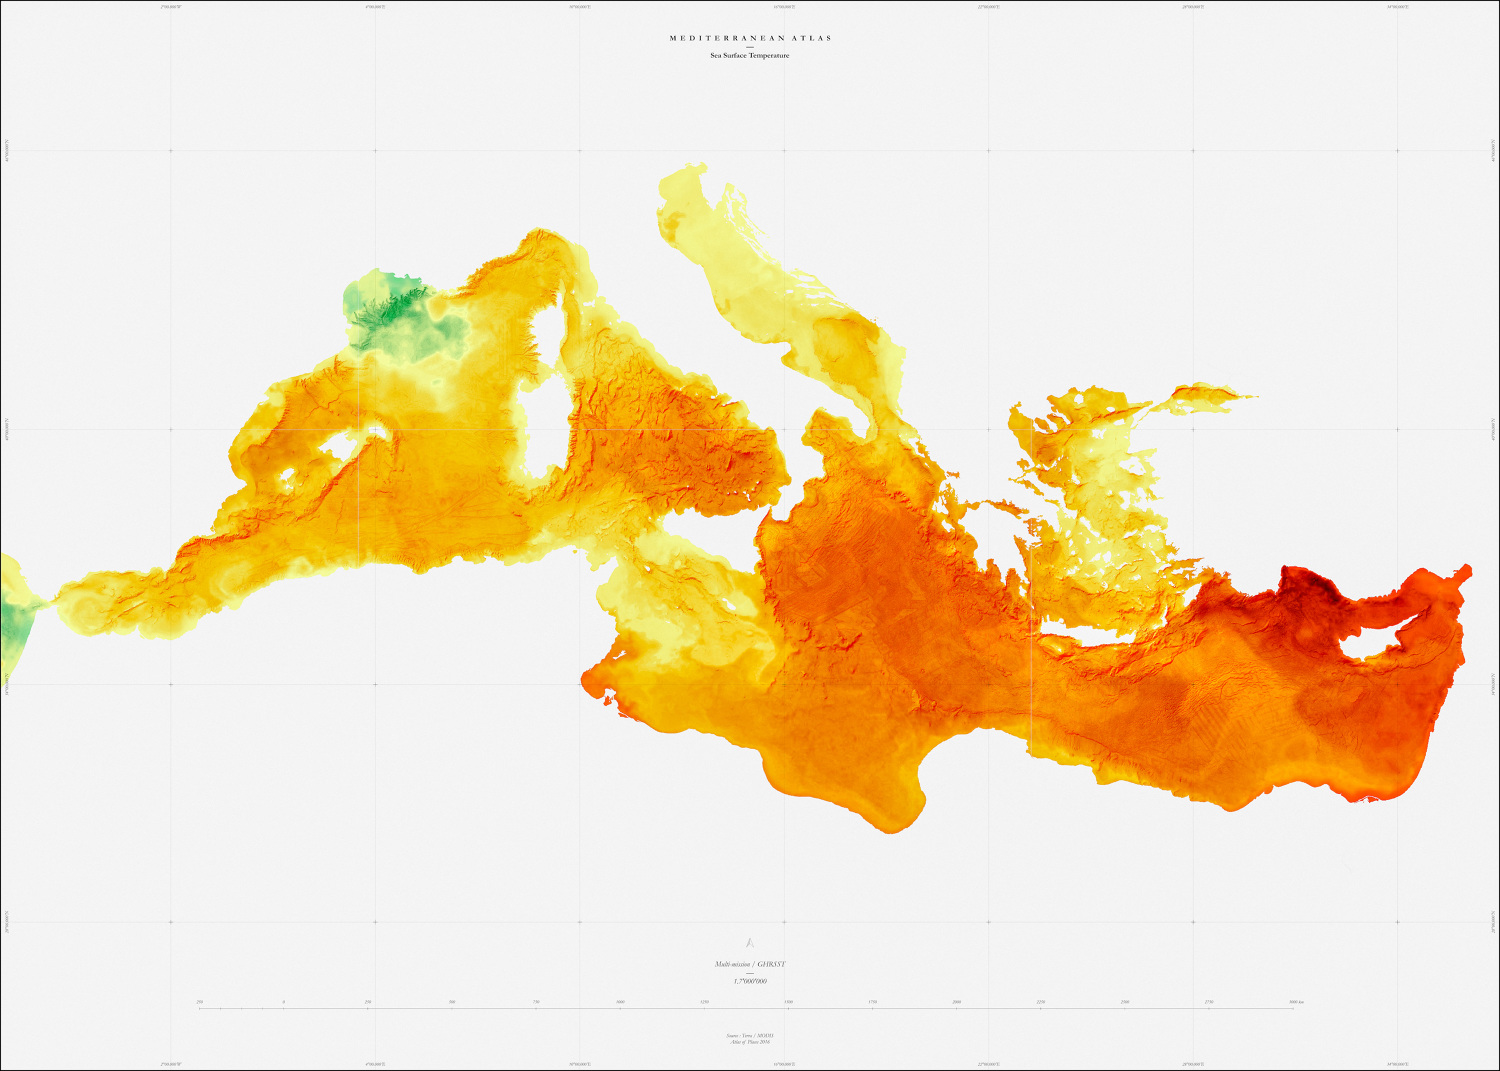
\includegraphics[width=0.8\textwidth]{MEDITERRANEAN_ATLAS_06_V3_1500.jpg} \\ }
   \only<1>{\textcolor{gris}{\href{https://atlasofplaces.com/research/mediterranean-sea-collection/}{Source: Atlas of places}}}
   \only<2>{\centering 
\includegraphics[width=0.5\textwidth]{M5-Flag_of_the_United_Nations.png} \\ }
   \only<2>{\textcolor{gris}{\href{https://en.wikipedia.org/wiki/Flag_of_the_United_Nations}{Flag of the United Nations \\ (Polar azimuthal equidistant projection.)}}}
   \only<3>{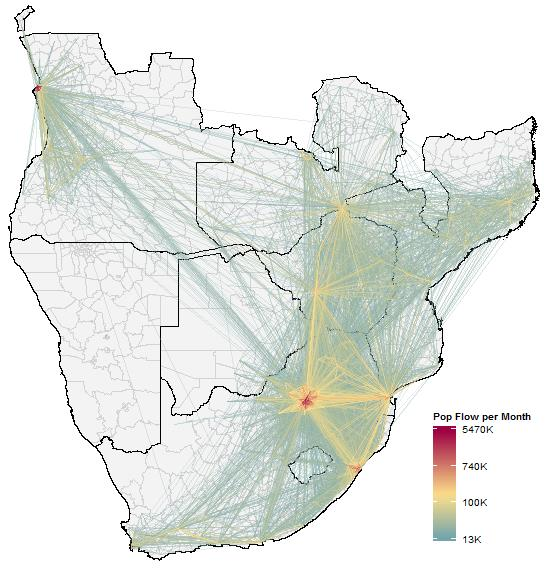
\includegraphics[width=0.5\textwidth]{M5-Flows-Mobile.jpg} \\ }
   \only<3>{\textcolor{gris}{\href{https://www.worldpop.org/focus_areas\#case3}{Source: World Pop}}}
   \only<4>{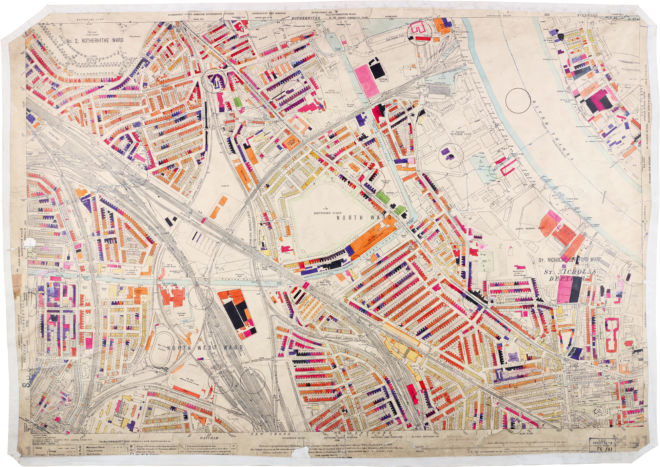
\includegraphics[width=0.5\textwidth]{LondonDammagesWWII.jpg} \\ }
   \only<4>{\textcolor{gris}{\href{http://phenomena.nationalgeographic.com/2016/05/18/bomb-damage-maps-reveal-londons-world-war-ii-devastation/}{The London County Council Bomb Damage Maps, 1939-1945-  Source: National Geographic}}}
   %\only<5>{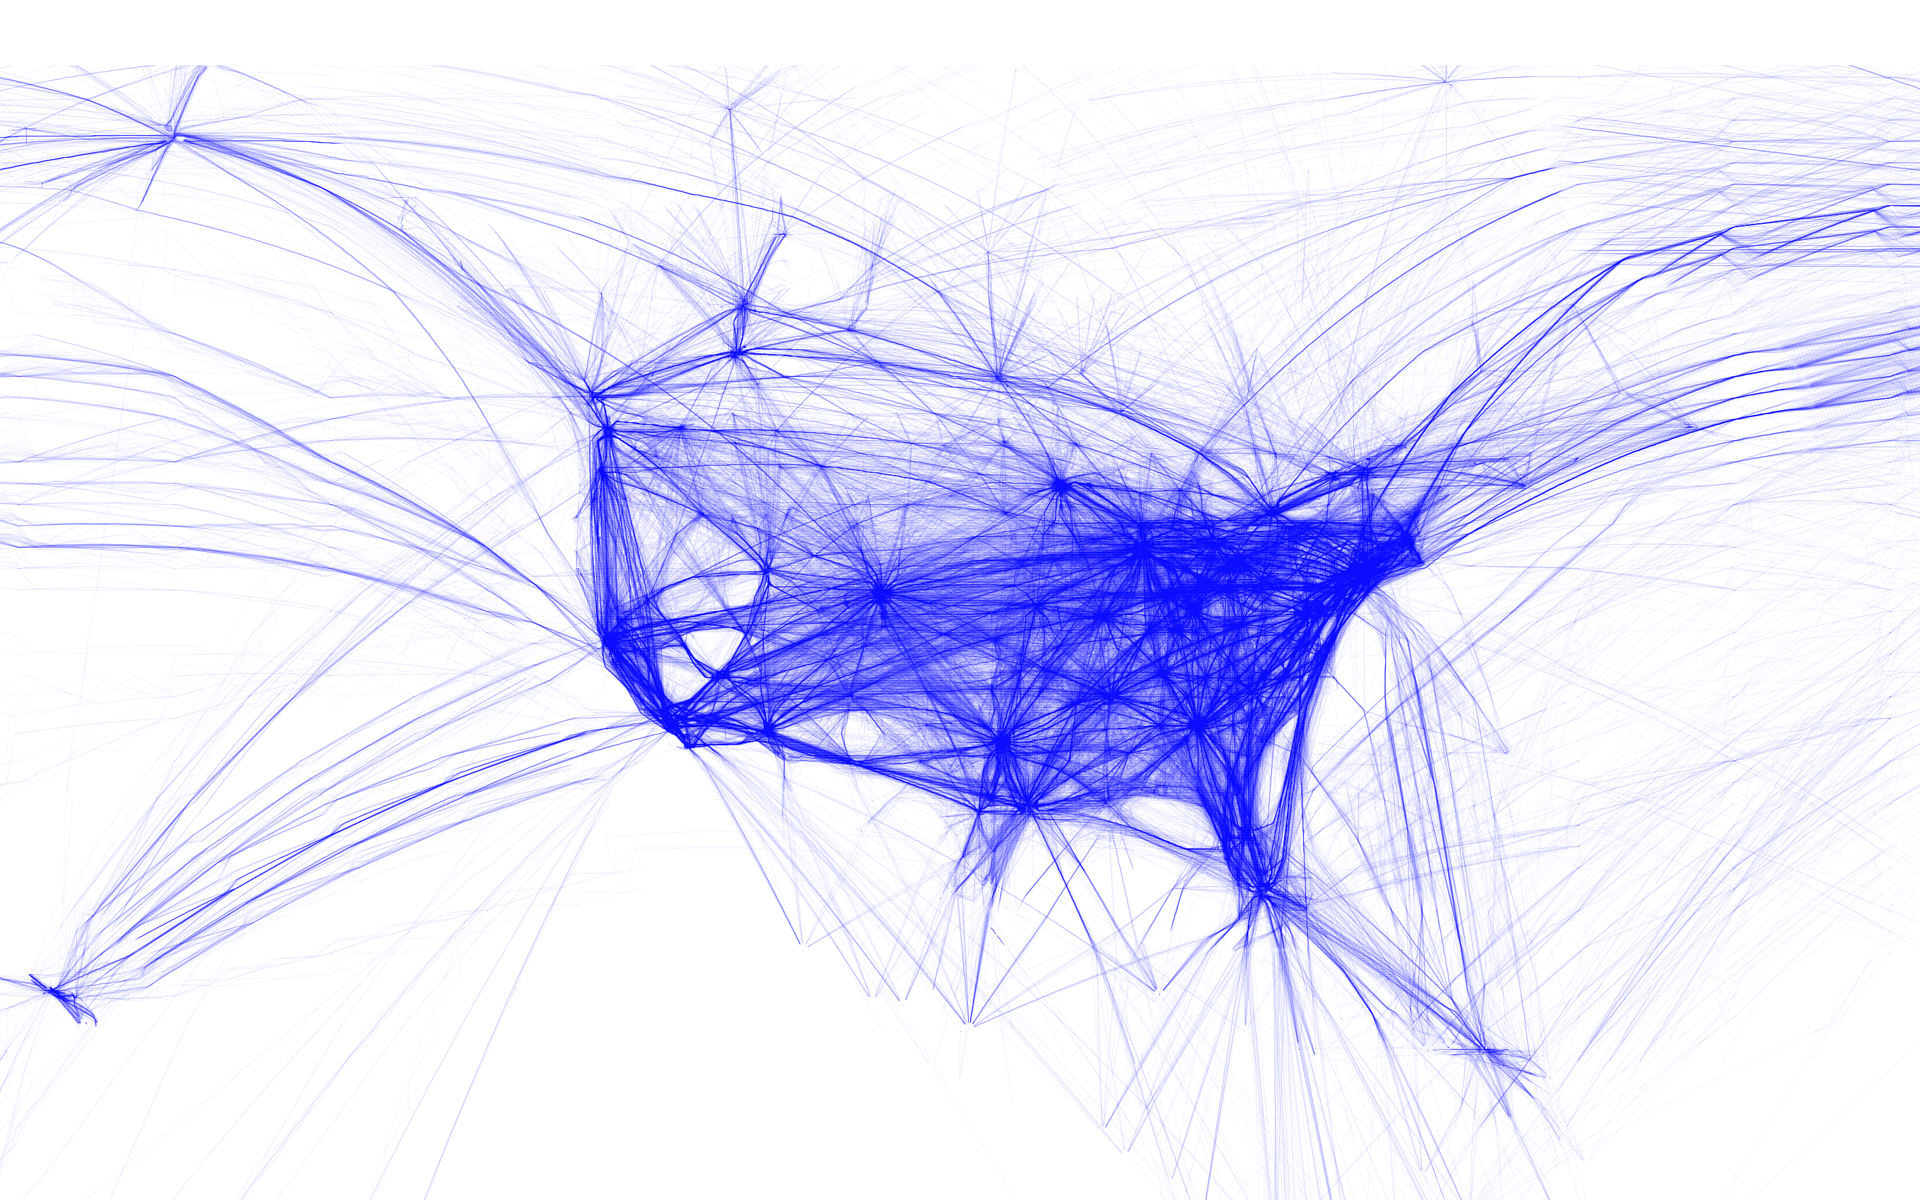
\includegraphics[width=1.0\textwidth]{Koblin.png} \\}
%   \only<5>{\textcolor{gris}{\href{http://www.aaronkoblin.com/work/flightpatterns}{Source: Aaron Koblin}}}
\end{itemize}
\end{center}
\end{frame}

\section{Statistical Maps}

\begin{frame} % Cover slide
\frametitle{\textcolor{brique}{[-  \textbf{Statistical Maps} -]}}
Visual representation of (geographical) information
\begin{itemize}[<+-|alert@+>]
    \item A (statistical) map is also \textbf{a visual representation}  of data
    \item A (statistical) map  can also be \textbf{a visual summary} of data
   % \item Maps are encoded using Bertin's visual variables
    \item Very technical domain of data visualization
    \item Questions addressed to maps are of spatial nature
    \item  \textbf{Many rules} for drawing a map!
    %\item  Maps are projections
\end{itemize}
\end{frame}

\begin{frame} % Cover slide
\frametitle{\textcolor{brique}{[- \textbf{Maps are projections} -]}}
\begin{center}
\begin{itemize}
   \only<1>{  \href{https://thetruesize.com}{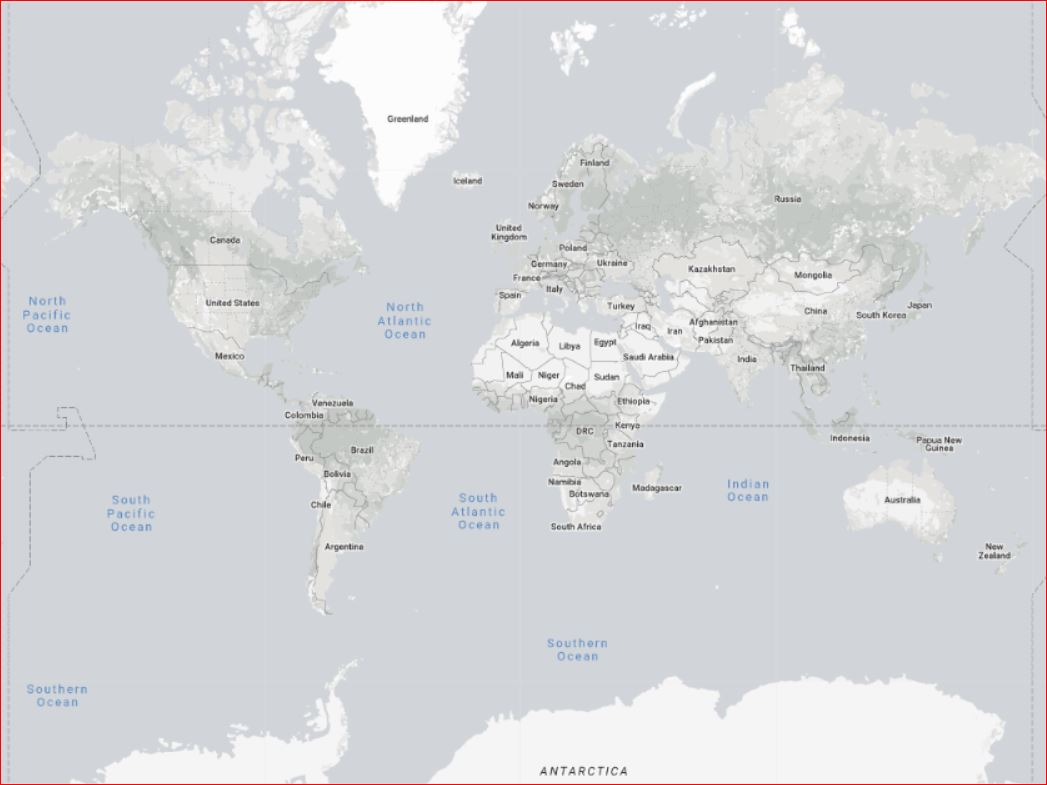
\includegraphics[width = 0.8\textwidth]{WorldMercator0.JPG}} \\ }
   \only<2>{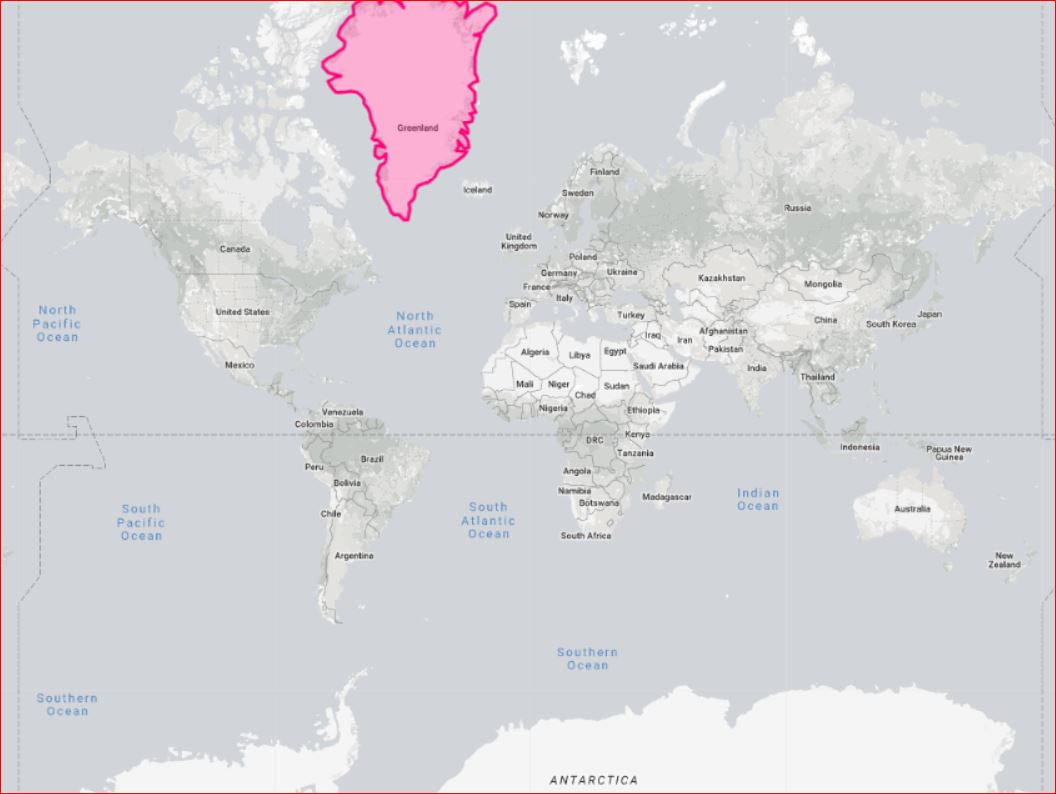
\includegraphics[width = 0.8\textwidth]{WorldMercatorGreenland0.JPG} \\ }
   \only<3>{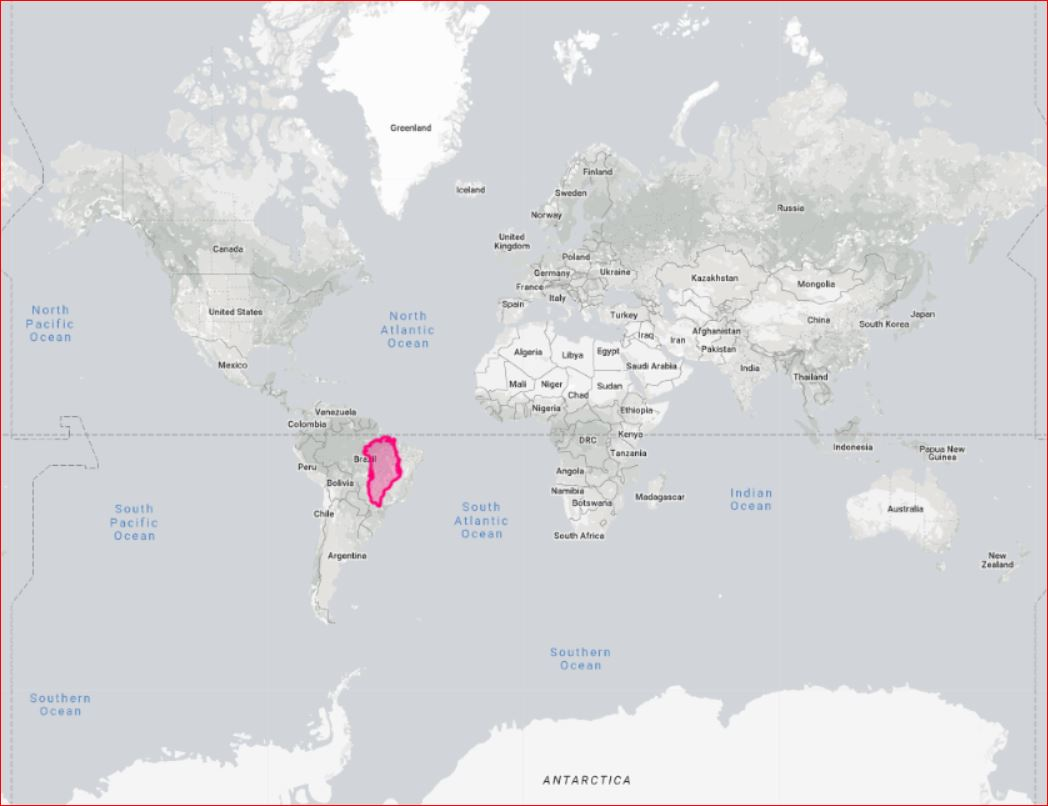
\includegraphics[width = 0.8\textwidth]{WorldMercatorGreenland0Brazil.JPG} \\ }
   \only<1-3>{\textcolor{gris}{\footnotesize{Source: \href{https://thetruesize.com}{https://thetruesize.com}}} \\ }
   \only<4>{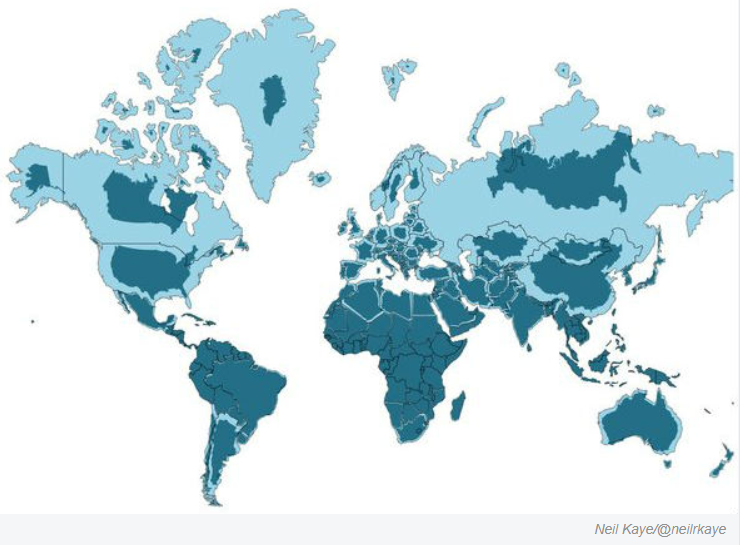
\includegraphics[width = 0.7\textwidth]{M5-Mercator.PNG} \\ }
   \only<4>{\textcolor{gris}{\footnotesize{Source: \href{https://www.reddit.com/r/dataisbeautiful/comments/9nkhkz/animating_the_mercator_projection_to_the_true/}{Neil Kaye}}}}
 %  \only<5>
 %  \only<5>
\end{itemize}
\end{center}
\end{frame}

%\begin{frame} % Cover slide
%\frametitle{\textcolor{brique}{[-  \textbf{Maps have limitations} -]}}
%\begin{itemize}[<+-|alert@+>]
%    \item  Limited choice  for  \textbf{efficient} visual variables
%    \item[] 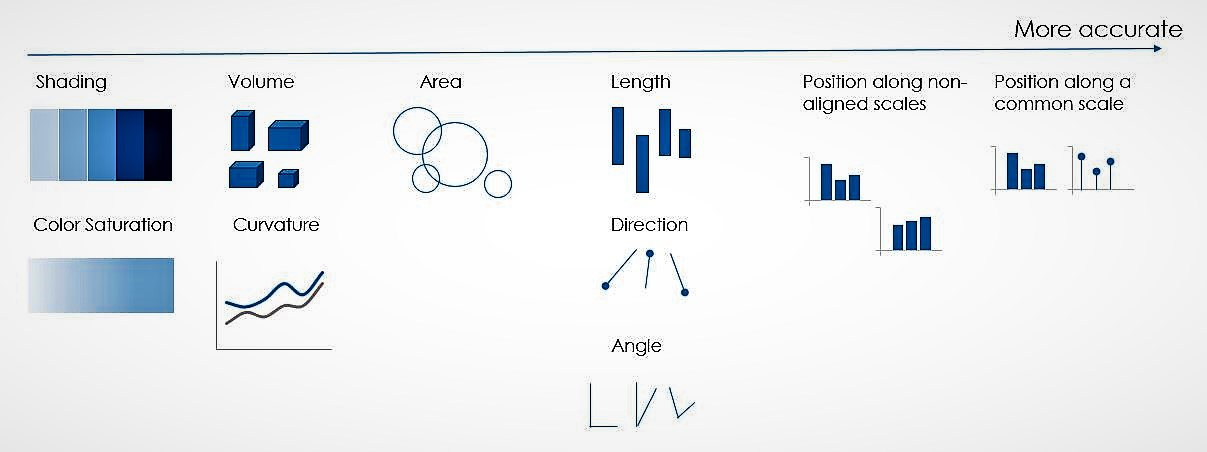
\includegraphics[width = 0.85\textwidth]{M2-Cleveland-and-McGillHorizontalNew.jpg}
%    \item[] {\textcolor{gris}{\footnotesize{Cleveland \& McGill Scale}}}
%    \item  Position (X-Y), order, size, shapes imposed
%    \item  Only colors \& objects shapes
%\end{itemize}
%\end{frame}

\begin{frame}
\frametitle{\textcolor{brique}{[-  \textbf{Maps have limitations} -]}}
    \begin{columns}
        \column{0.4\textwidth}
            \begin{itemize}[<+->]
                \item Only \textbf{one} variable
                \item Comparable neighbours
                \item Choosing the right palette
                \item Choosing the right encoding
                \item Choosing the right graphic
            \end{itemize}
        \column{0.6\textwidth}
            \only<1>{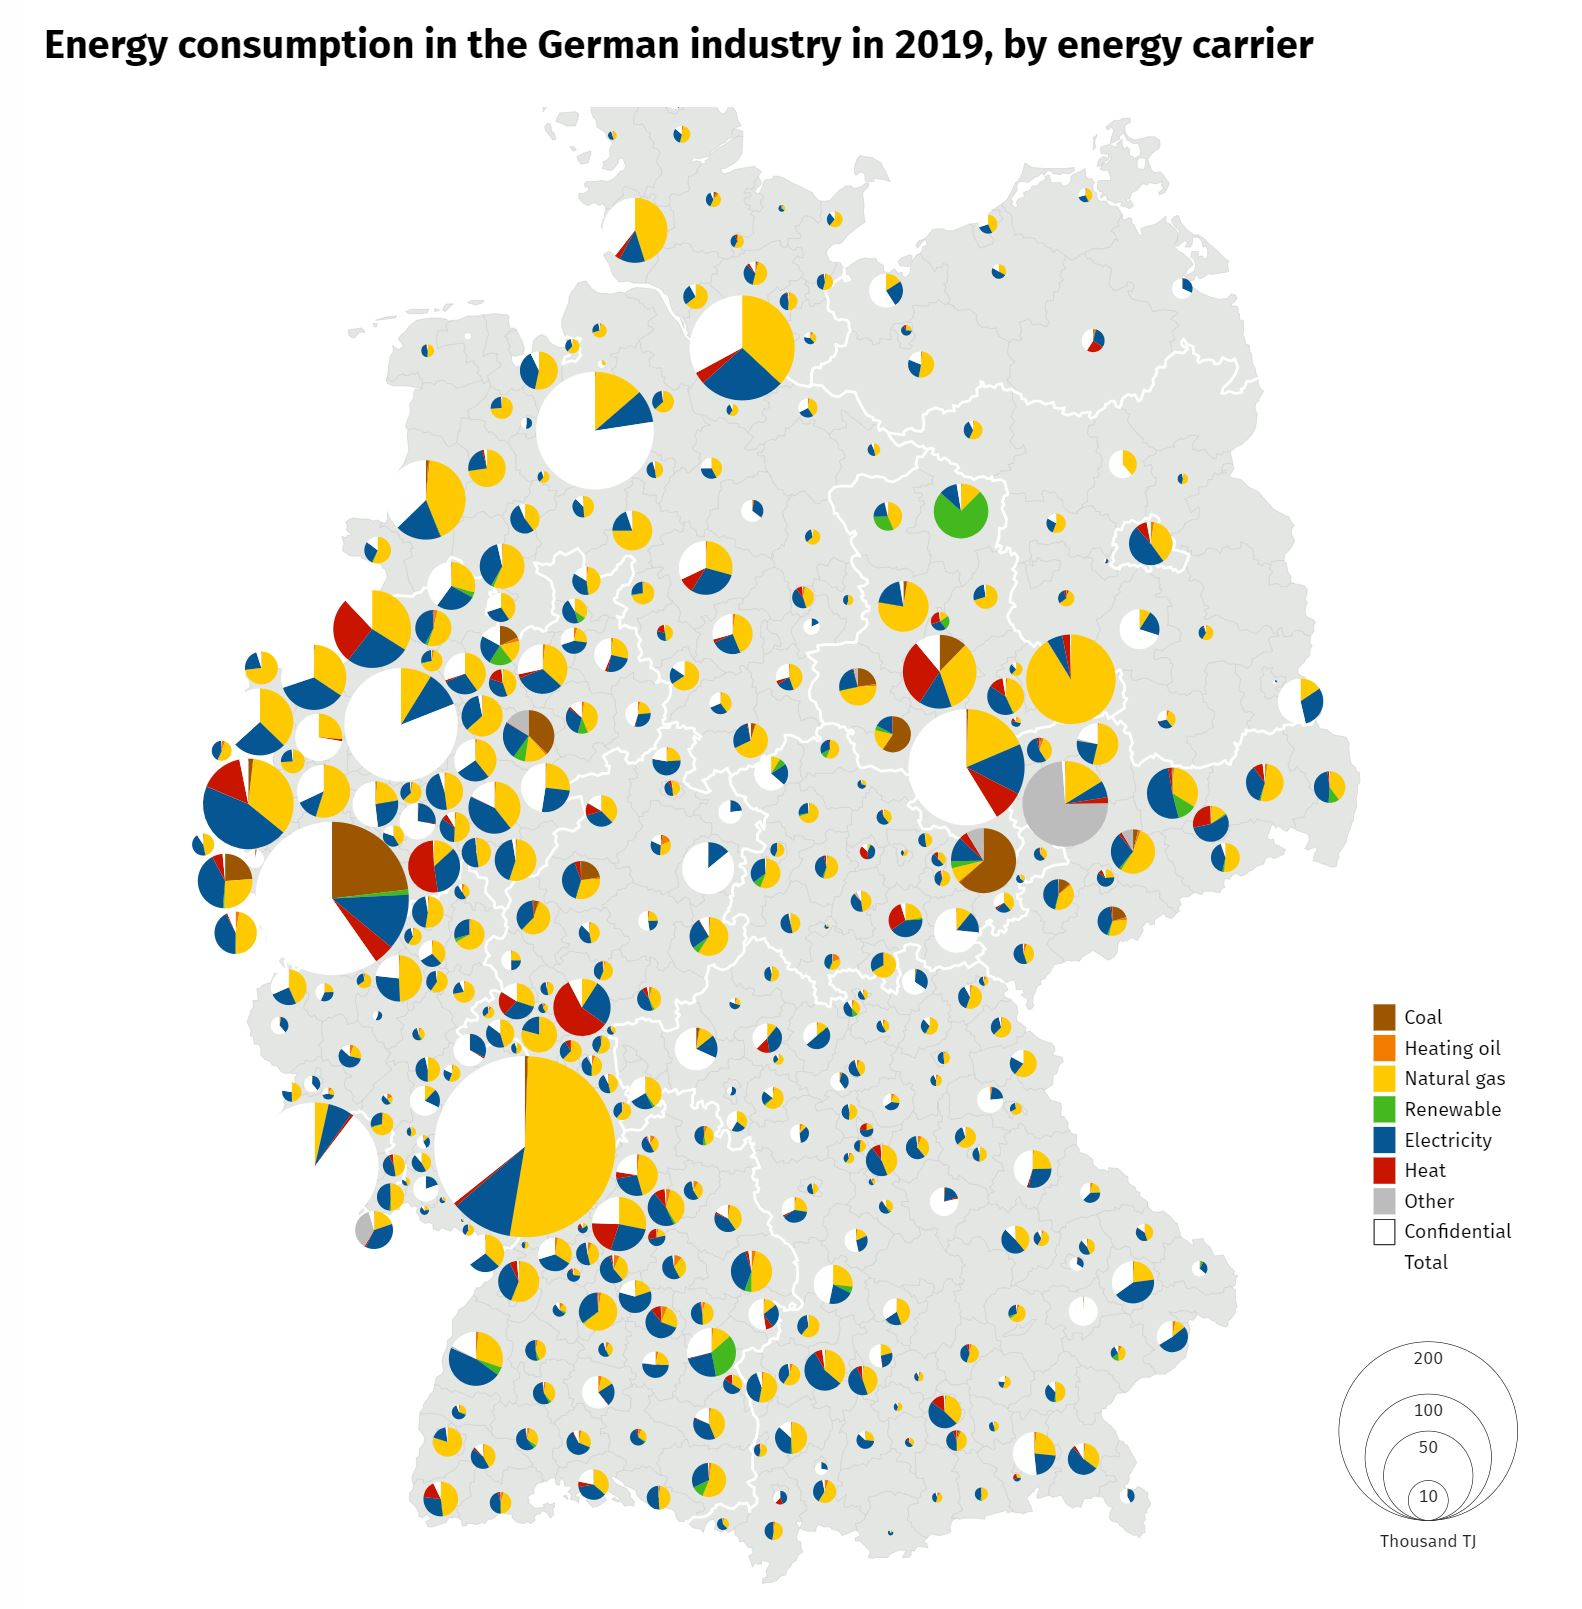
\includegraphics[width = 0.8\textwidth]{BadGermanyMapwithPies.JPG} \\ }
            \only<1>{\textcolor{gris}{\footnotesize{\href{https://www.destatis.de/EN/Press/2020/12/PE20_476_435.html}{Statistisches Bundesam}}}}
            \only<2>{\href{https://ourworldindata.org/grapher/women-political-empowerment-index}{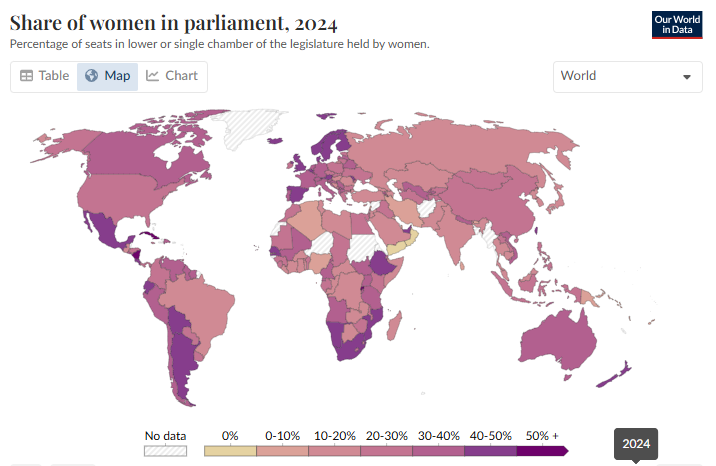
\includegraphics[width=1.0\textwidth]{ShareWomenParliament-map.png}} }
            \only<2>{\textcolor{gris}{\footnotesize{\href{https://ourworldindata.org/grapher/women-political-empowerment-index}{Our World in Data}}}}
            \only<3>{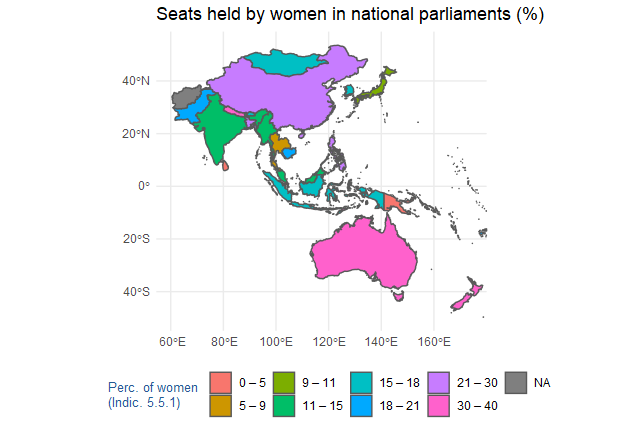
\includegraphics[width=1.0\textwidth]{ShareWomenParliamentChoro1.png} }
            \only<4>{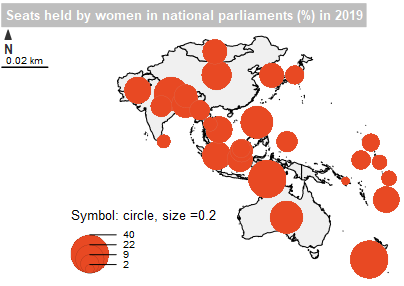
\includegraphics[width=1.0\textwidth]{ShareWomenParliamentSymb-Big.png} }
            \only<5>{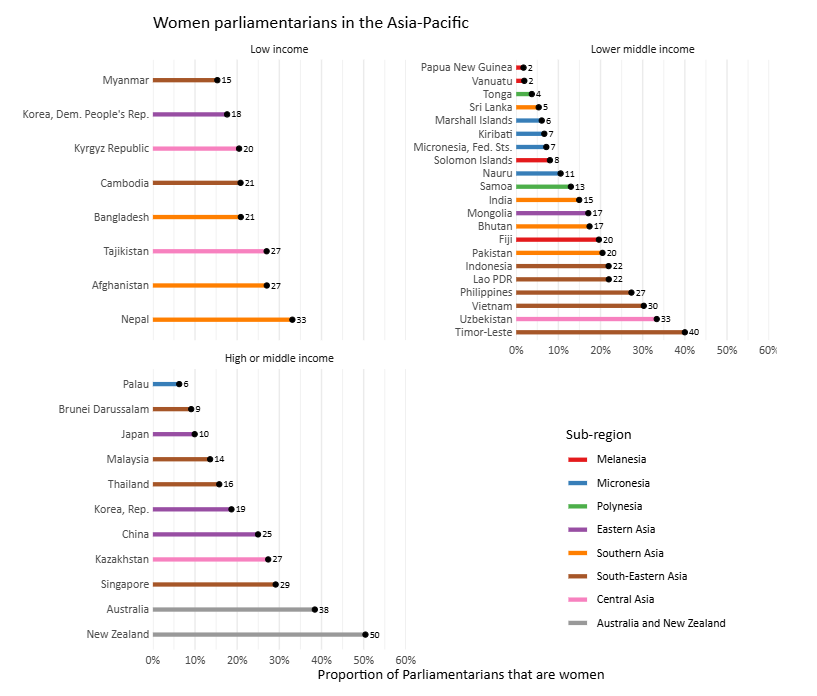
\includegraphics[width=1.0\textwidth]{ShareWomenParliament-BarChart.png} }
            \only<5>{\textcolor{gris}{\footnotesize{\href{https://freerangestats.info/blog/2023/05/26/women-parl-map}{Free Range Statistics}}}}
    \end{columns}
\end{frame}

\section{Choropleth}

\begin{frame} % Cover slide
\frametitle{\textcolor{brique}{[-  \textbf{Choropleth Maps} -]}}
\begin{itemize}[<+-|alert@+>]
    \item  Used to show regional pattern in data   % https://storymaps.arcgis.com/collections/04a7887dd16343c384ef1963fc06fdb5?item=3
    \item  Good for the big picture, not for details
    \item  Work best for relative (to population) numbers
    \item  Choice of the right color scheme
    \item  Choice of the right palette % (https://gka.github.io/palettes)
    \item  Follow Choropleth maps rules % (https://blog.datawrapper.de/choroplethmaps/)
\end{itemize}
\end{frame}



\begin{frame} % Cover slide
\frametitle{\textcolor{brique}{[-  \textbf{Colors on Maps} -]}}
\begin{center}
\begin{itemize}
   \only<1>{Choice of \textit{color\textbf{s}} is really important \\ }
   \only<1>{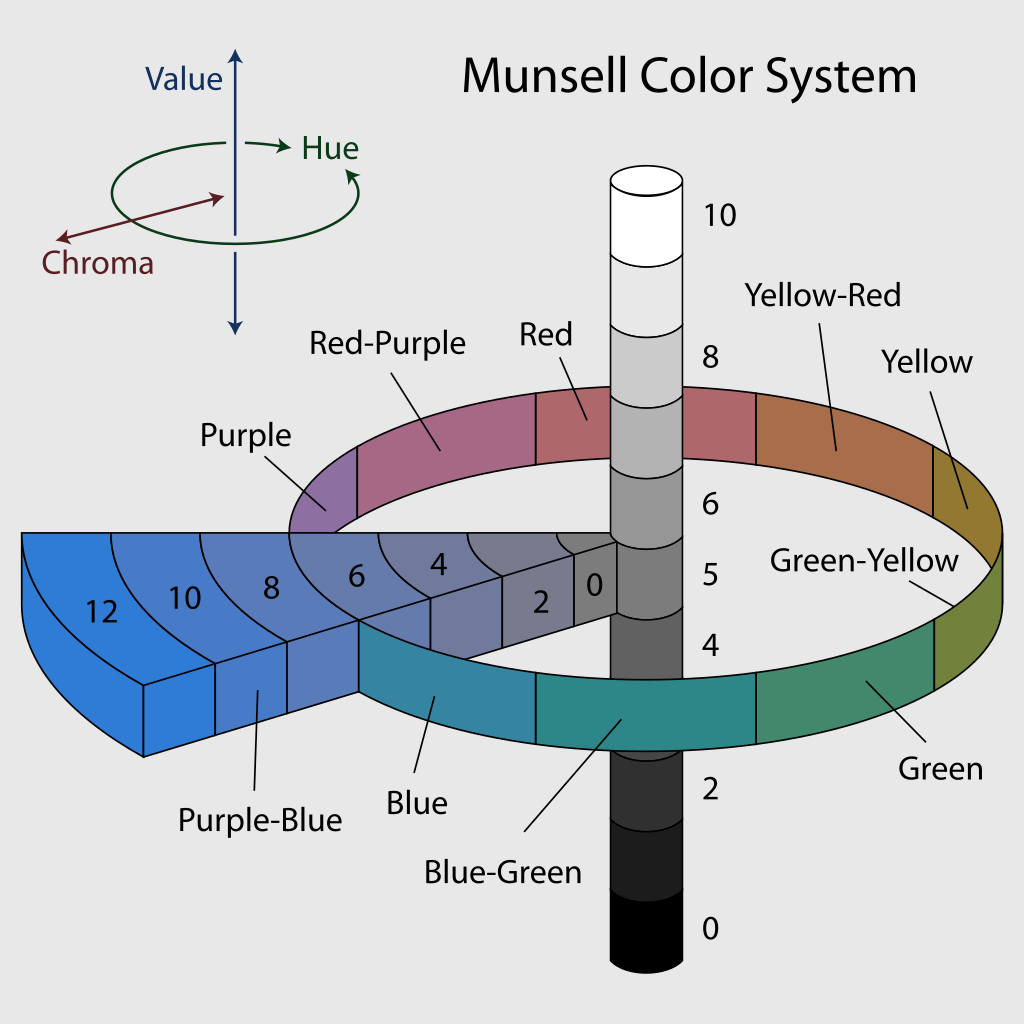
\includegraphics[width = 0.4\textwidth]{Color-Munsell-system.Wikipedia.png} \\ }
   \only<1>{\textcolor{gris}{\footnotesize{Munsell color system. Source: \href{https://en.wikipedia.org/wiki/Munsell_color_system}{ Wikipedia}}} \\ }
   \only<2>{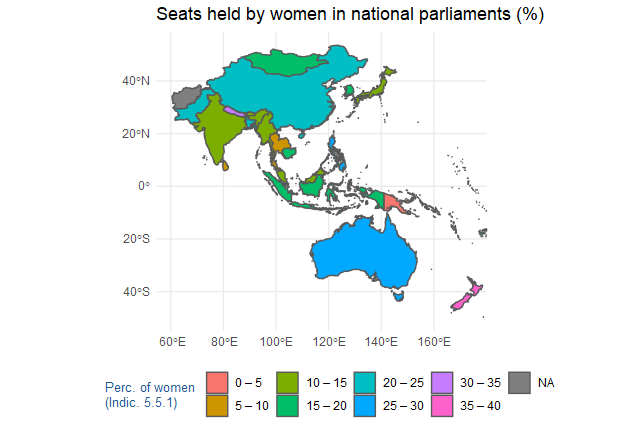
\includegraphics[width = 0.7\textwidth]{ShareWomenParliamentChoro2.png} \\ }
   \only<3>{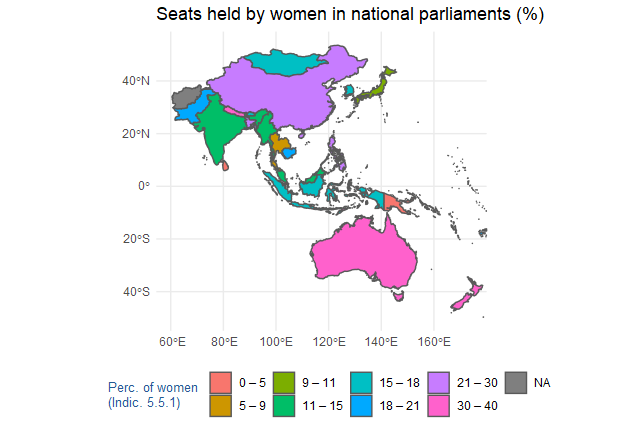
\includegraphics[width = 0.7\textwidth]{ShareWomenParliamentChoro1.png} \\ }
   \only<4>{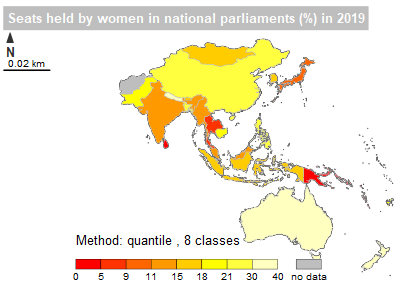
\includegraphics[width = 0.7\textwidth]{ShareWomenParliamentChoroCont.png} \\ }

    \end{itemize}
\end{center}
\end{frame}

\begin{frame} % Cover slide
\frametitle{\textcolor{brique}{[-  \textbf{Color classification considerations} -]}}
{\centering

\includegraphics[width = 0.8\textwidth]{M5-ColorBlindPalette.JPG}
} \\
Color palette: \\
\vspace{0.5cm}
\begin{itemize}[<+-|alert@+>]
    \item  Must be chosen with a reason
    \item  Must be chosen  by a human (not a software)
    \item  Can use descriptive statistics (min, max, skew)
    \item  Should be based on subject matter
    \item  Should help the comparison
    \item  Should be accessible to all (colorblind)
\end{itemize}
\end{frame}


%\begin{frame} % Cover slide
%\frametitle{\textcolor{brique}{[-  \textbf{Population Density in France} -]}}
%\begin{center}
%\begin{itemize}
%   \only<1-3>{ - Representing Population density on a Map \\ }
%   \only<2-3>{ - Continuous variable with many values (no "natural" classes of values) \\ }
%   \only<3>{ - Choice of colors \textbf{and} classes is important!}
%   \only<4>{Qualitative palette: bad choice}
%   \only<4>{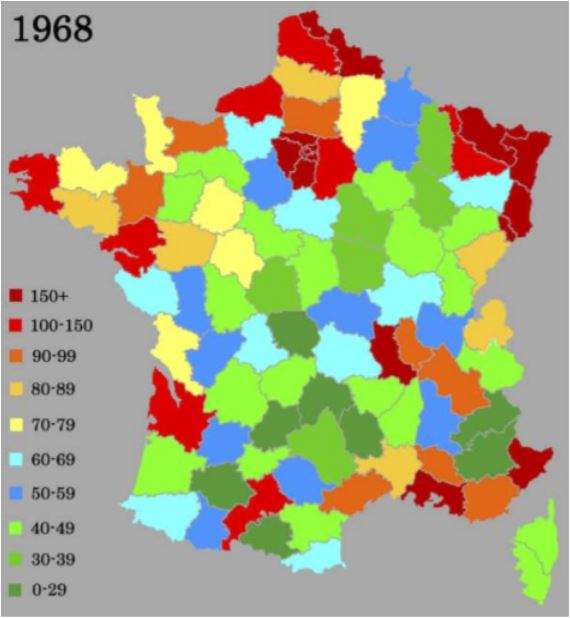
\includegraphics[width = 0.5\textwidth]{Colorfull-France.jpg} \\ }
%   \only<5>{Equal intervals: Sensitive to outliers  \\}
%   \only<5>{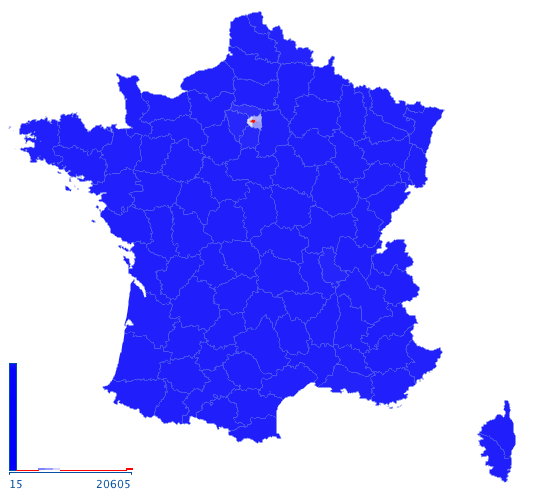
\includegraphics[width = 0.6\textwidth]{FrancePopLinear.png} \\ }
%   \only<6>{Non linear intervals with several hues \\}
%   \only<6>{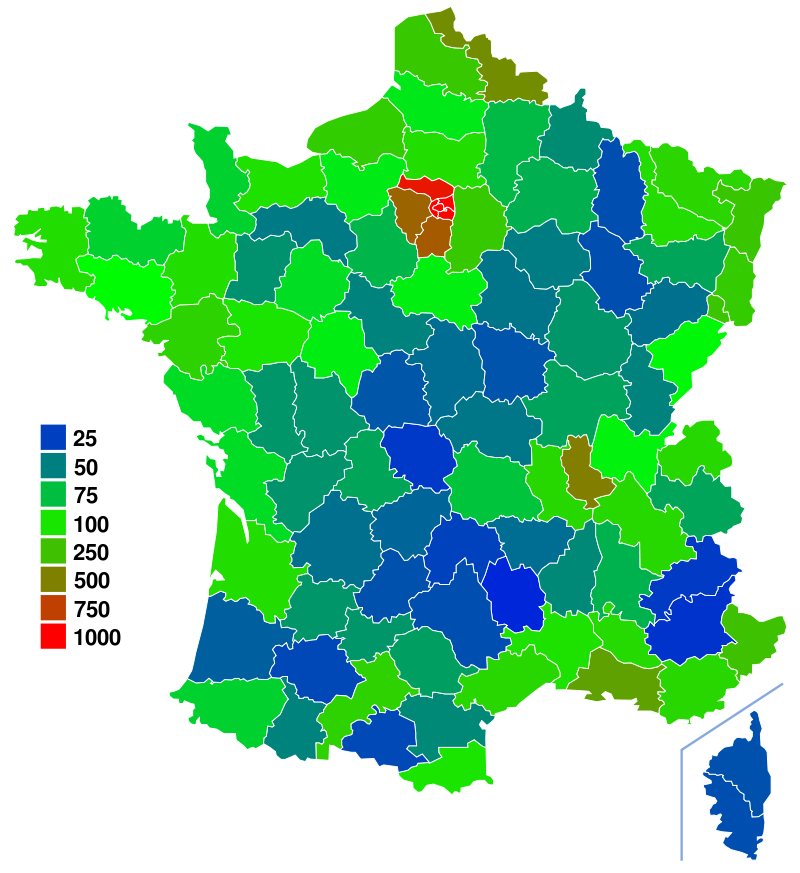
\includegraphics[width = 0.5\textwidth]{FranceDensitePopulationNonLinear.png} \\ }
%   \only<5-6>{\textcolor{gris}{\footnotesize{Population density. Source: \href{https://en.wikipedia.org/wiki/Demographics_of_France}{Wikipedia}}} \\ }
%   \only<7>{Non linear intervals: Bi-polar progression \\}
%   \only<7>{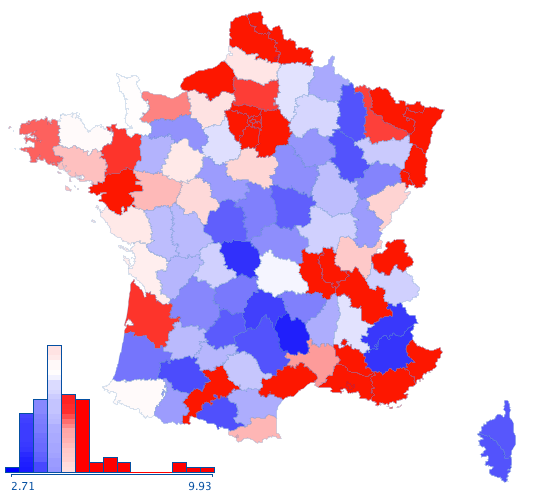
\includegraphics[width = 0.6\textwidth]{FranceCutOff.png} \\ }
%   \only<8>{Non linear intervals: Bi-polar progression modified \\}
%   \only<8>{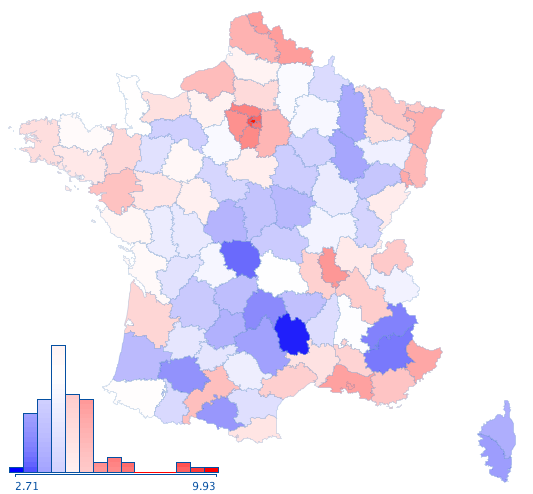
\includegraphics[width = 0.6\textwidth]{FranceTheGood.png} \\ }
%   \only<9>{Non linear intervals: Single hue progression \\}
%   \only<9>{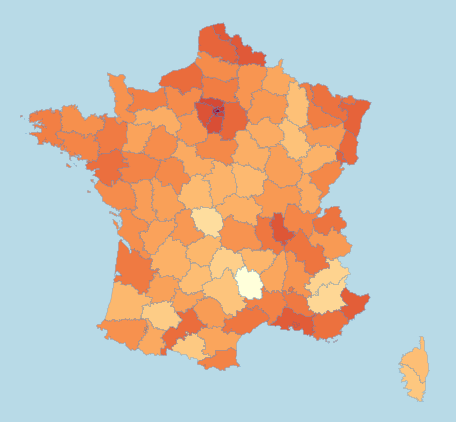
\includegraphics[width = 0.6\textwidth]{FranceComment.png} \\ }
%   \only<7-9>{\textcolor{gris}{\footnotesize{Population density. Source: \href{https://www.theusrus.de/blog/the-good-the-bad-22012/}{ Martin Theus}}} \\ }
%   \only<10>{Single hue progression with smaller administrative units \\}
%   \only<10>{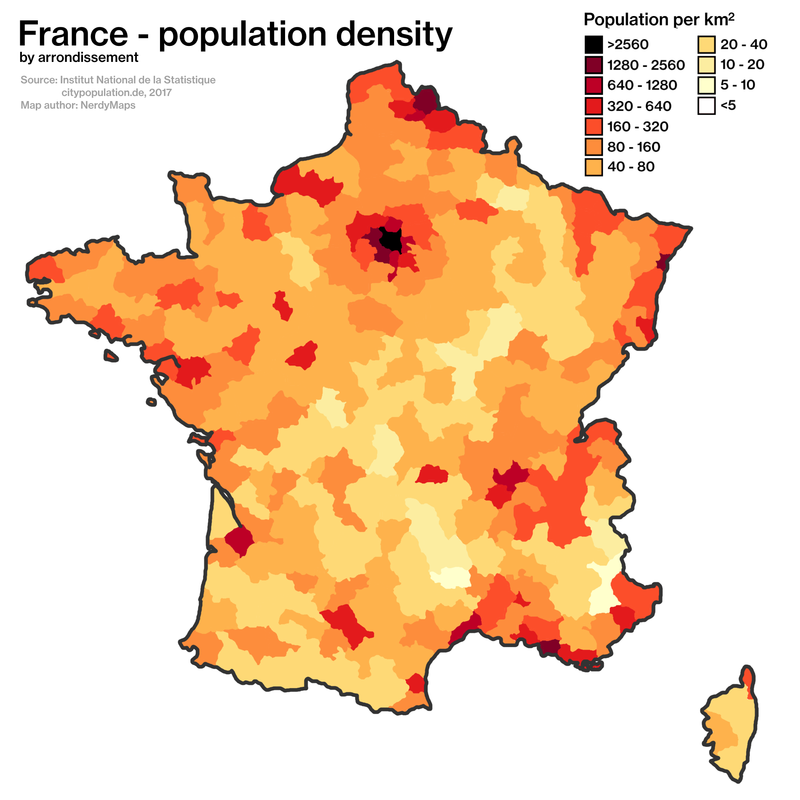
\includegraphics[width = 0.6\textwidth]{FranceModern.png} \\ }
%   \only<11>{Single hue progression with smaller administrative units \\}
%   \only<11>{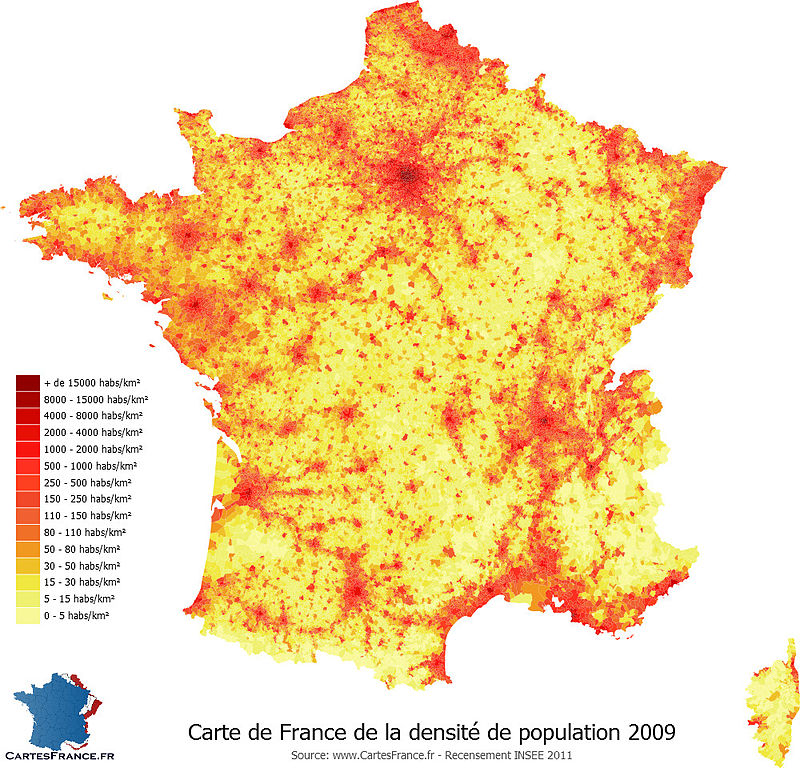
\includegraphics[width = 0.6\textwidth]{France_density_2009.jpg} \\ }
%   \only<10-11>{\textcolor{gris}{\footnotesize{Population density. Source: \href{https://en.wikipedia.org/wiki/Demographics_of_France}{Wikipedia}}} \\ }
%\end{itemize}
%\end{center}
%\end{frame}
%
%\begin{frame} % Cover slide
%\frametitle{\textcolor{brique}{[-  \textbf{Population Density in France} -]}}
%Pattern recognition differs with maps
%\begin{center}
%\begin{itemize}
%  \item[]   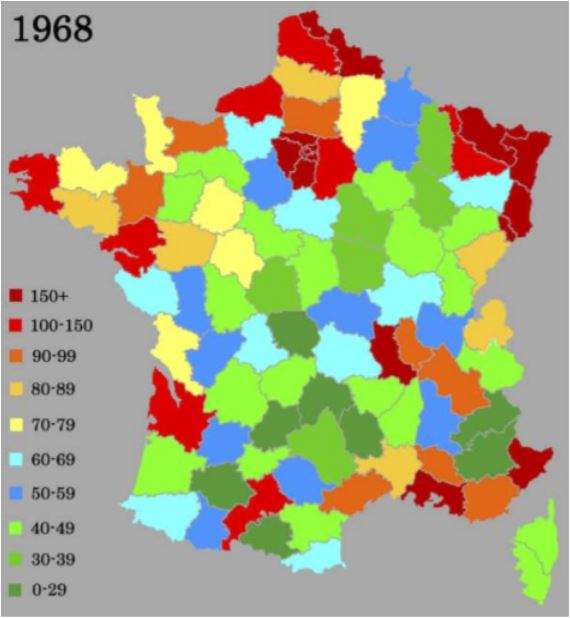
\includegraphics[width = 0.2\textwidth]{Colorfull-France.jpg}
%            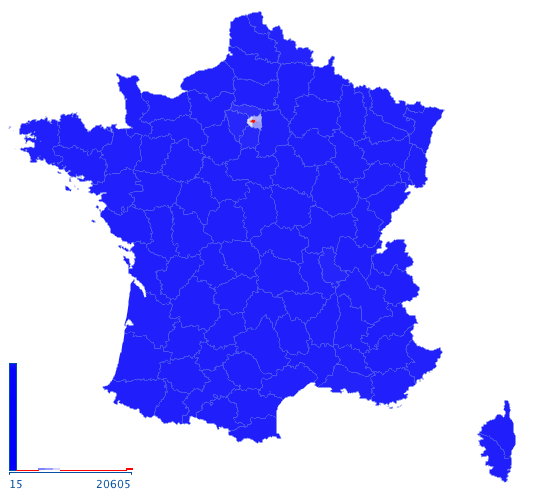
\includegraphics[width = 0.2\textwidth]{FrancePopLinear.png}
%            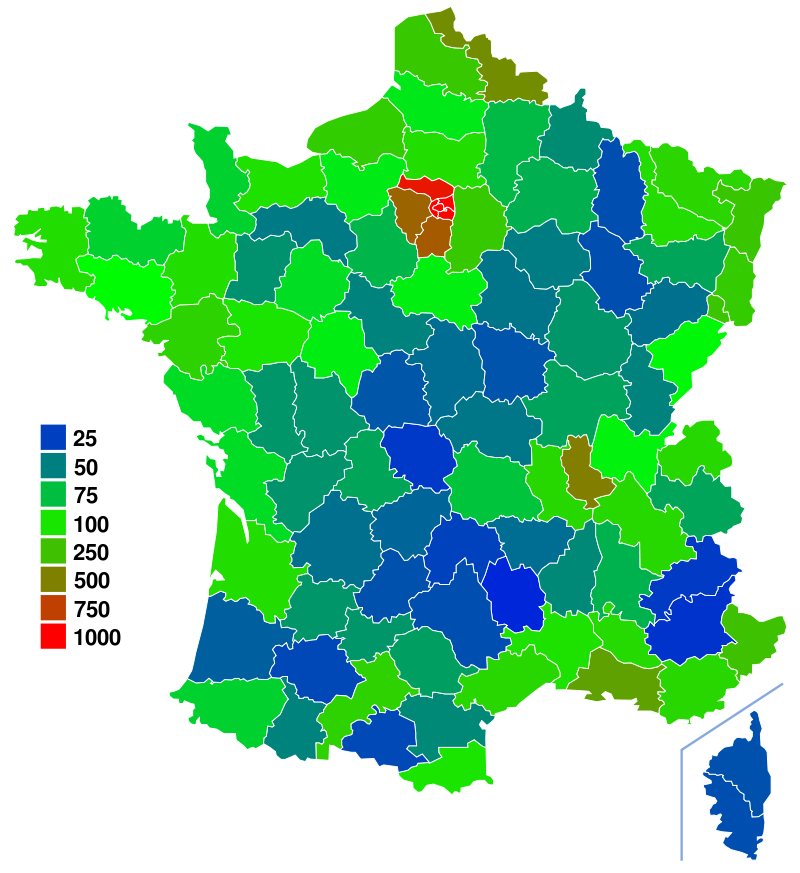
\includegraphics[width = 0.2\textwidth]{FranceDensitePopulationNonLinear.png}
%            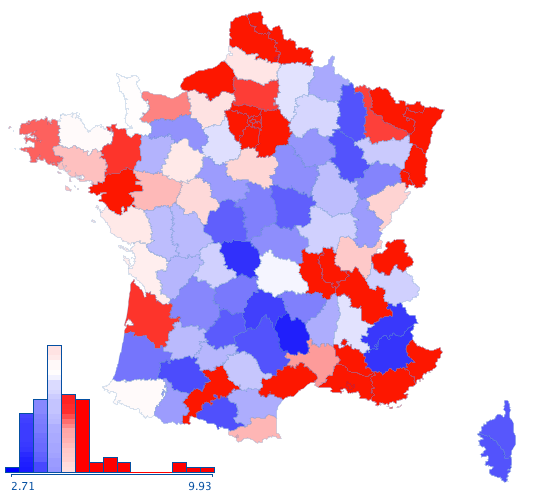
\includegraphics[width = 0.2\textwidth]{FranceCutOff.png}
%  \item[]   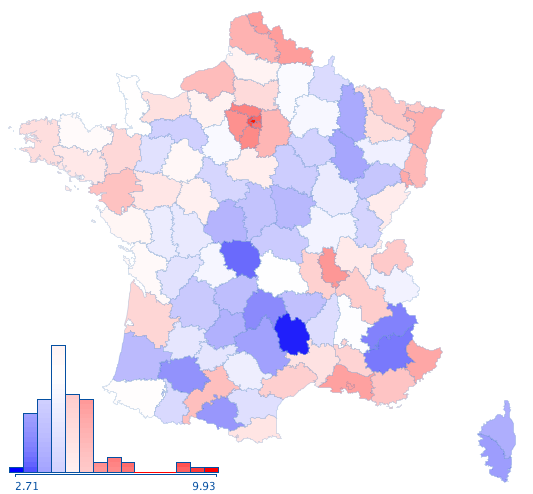
\includegraphics[width = 0.2\textwidth]{FranceTheGood.png}
%            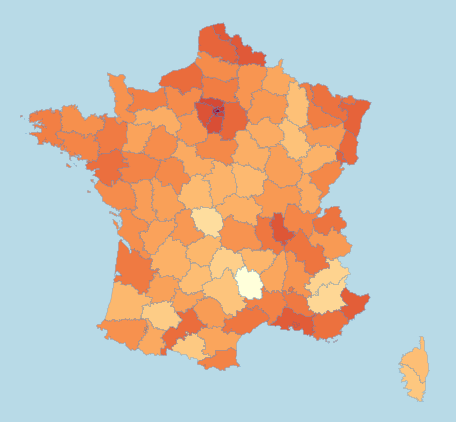
\includegraphics[width = 0.2\textwidth]{FranceComment.png}
%            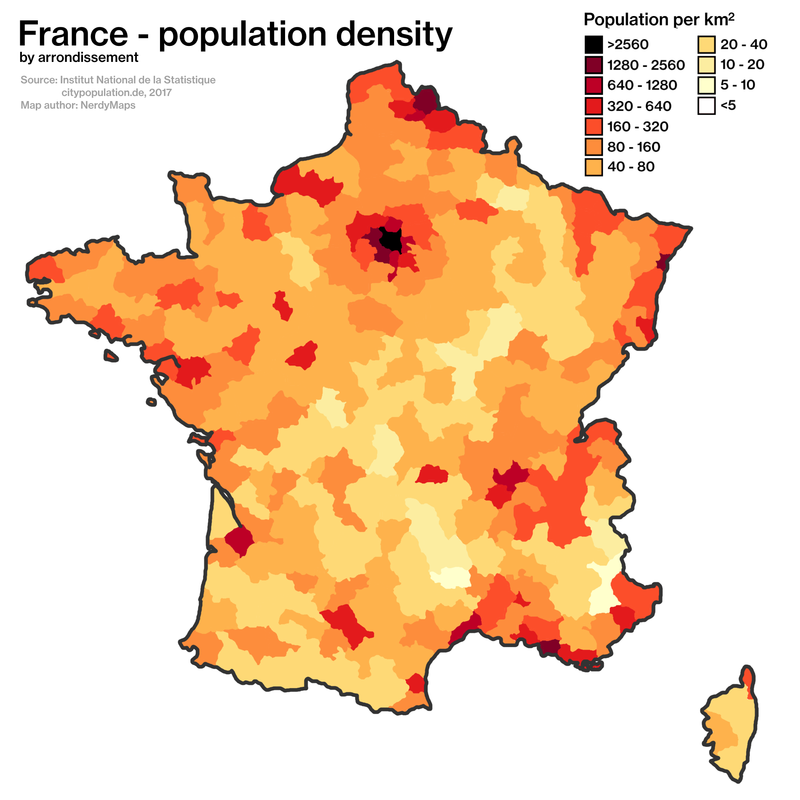
\includegraphics[width = 0.2\textwidth]{FranceModern.png}
%            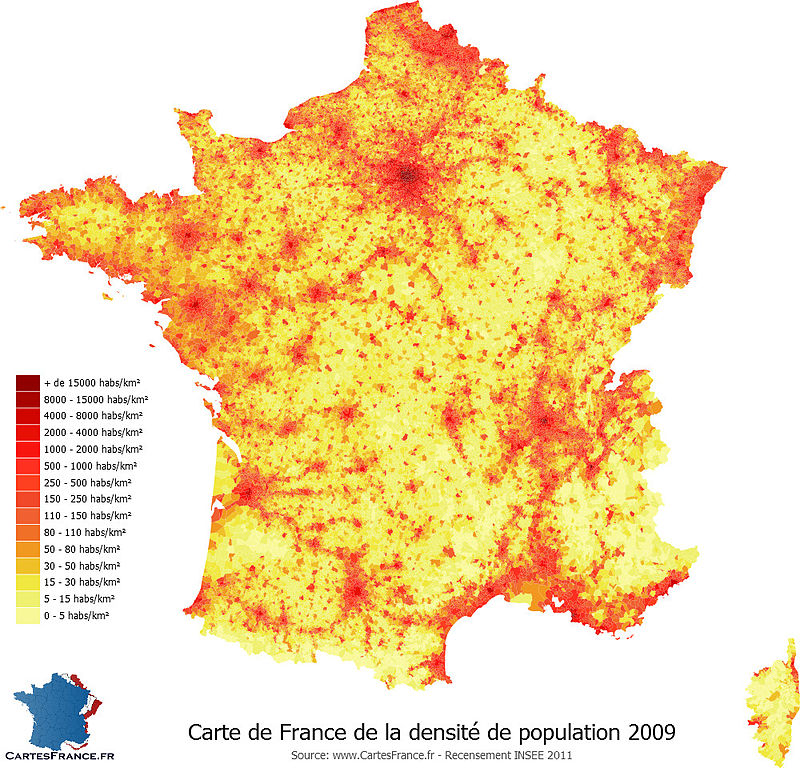
\includegraphics[width = 0.2\textwidth]{France_density_2009.jpg}
%\end{itemize}
%\end{center}
%\end{frame}


\begin{frame} % Cover slide
\frametitle{\textcolor{brique}{[-  \textbf{Colors Palettes:} Qualitative variables (Categories) -]}}
\begin{center}
\begin{itemize}[<+-|alert@+>]
    \item[] For \textbf{qualitative} (not ordered) variables \\ (\textit{e.g.} sex, land, politics,..)
    \item Qualitative values: \hfill 
\includegraphics[width = 0.8\textwidth]{M5-ColorPaletteQualitative.png}
    \item Qualitative values (spectral): \hfill 
\includegraphics[width = 0.8\textwidth]{M5-ColorPaletteFullSpectral.png}
    \item[] \textcolor{gris}{\footnotesize{Source \href{https://en.wikipedia.org/wiki/Choropleth_map}{Wikipedia: Choropleth}}}
\end{itemize}
\end{center}
\end{frame}


\begin{frame} % Cover slide
\frametitle{\textcolor{brique}{[-  \textbf{Colors Palettes:}  Continuous variables  -]}}
\begin{center}
\begin{itemize}[<+-|alert@+>]
    \item[] For \textbf{continuous} (ordered) variables  (\textit{e.g.} Shares, population, etc.)
    %\item Continuous values (spectral): \hfill 
\includegraphics[width = 0.8\textwidth]{M5-ColorPalettePartialSpectral.png}
    \item Continuous values: Single hue: \hfill 
\includegraphics[width = 0.8\textwidth]{M5-ColorPaletteSingleHue.png}
    \item Continuous values: Color intensity (gray): \hfill 
\includegraphics[width = 0.8\textwidth]{M5-ColorPaletteGreyscale.png}
    \item Continuous diverging values: Diverging hues (bi-polar): \hfill 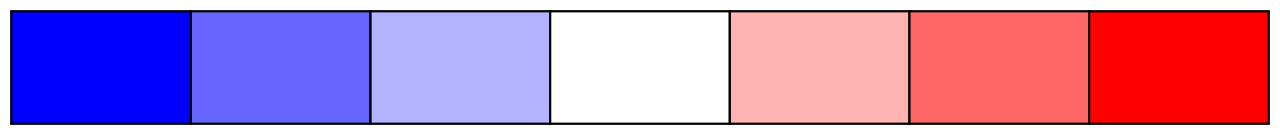
\includegraphics[width = 0.8\textwidth]{M5-ColorPaletteBiPolar.png}
  \item[] \textcolor{gris}{\footnotesize{Source \href{https://en.wikipedia.org/wiki/Choropleth_map}{Wikipedia: Choropleth}}}
\end{itemize}
\end{center}
\end{frame}


\begin{frame} % Cover slide
\frametitle{\textcolor{brique}{[-  \textbf{Colors for \textit{Choropleth} maps} -]}}
\begin{center}
\begin{itemize}
   \only<1>{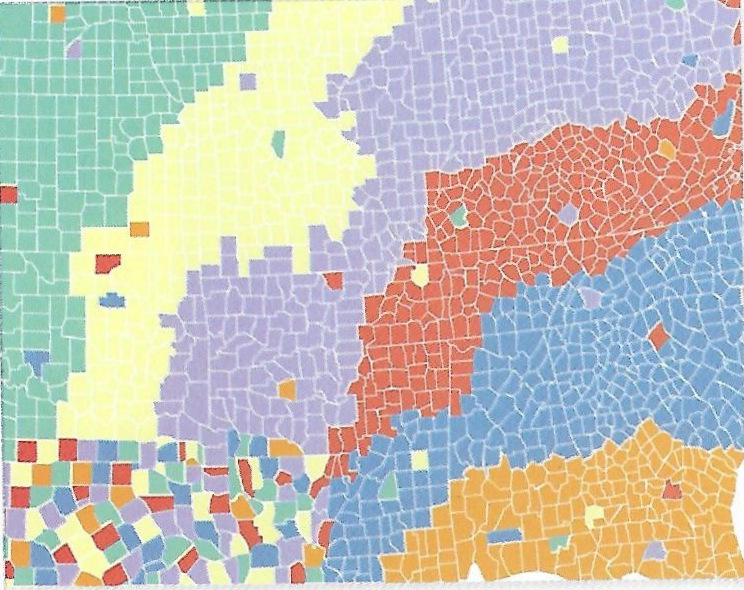
\includegraphics[width = 0.5\textwidth]{Yau-MapsColors-Qualitative.jpg} \\ }
   \only<1>{\footnotesize{For \textbf{qualitative} variables: Gender, land type, Religion.\\
                    $\hookrightarrow$ Different \textit{hues}} \\ }
   \only<2>{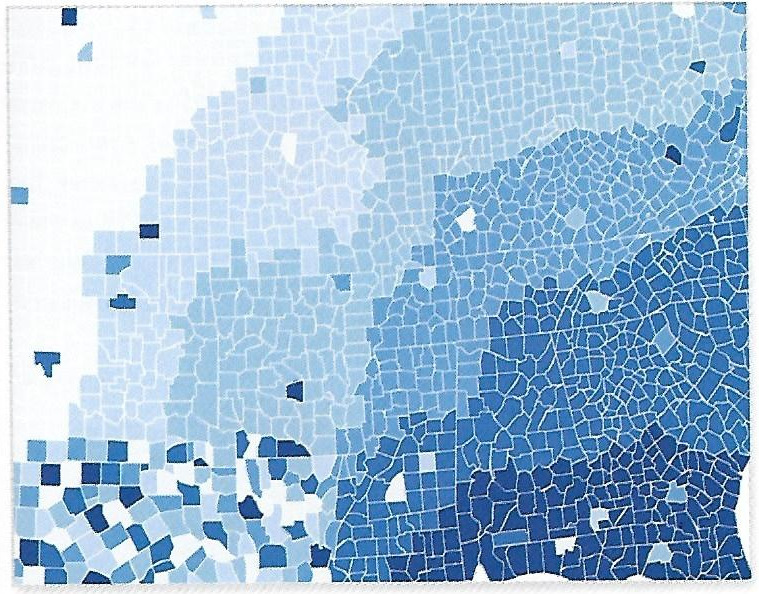
\includegraphics[width = 0.5\textwidth]{Yau-MapsColors-Sequential.jpg} \\ }
   \only<2>{\footnotesize{For "\textit{sequential}" \textbf{continuous} values: \emph{e.g.} Share of women who experienced violence, Poverty,share of women in parliament, ... \\
                    $\hookrightarrow$ Same hue, different intensity (chroma value)} \\}
   \only<3>{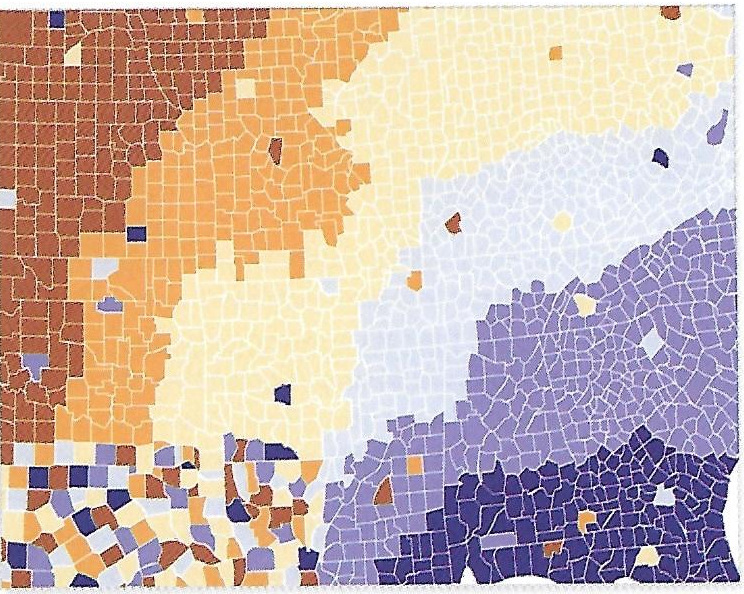
\includegraphics[width = 0.5\textwidth]{Yau-MapsColors-Diverging.jpg} \\ }
   \only<3>{\footnotesize{For "\textit{diverging}" \textbf{continuous} values: Changes in women's wealth (+/-), year to year comparison.\\
                        $\hookrightarrow$ Two hues, different intensity (chroma value)}\\ }
   \only<1-3>{\textcolor{gris}{\footnotesize{Source: \href{https://flowingdata.com/}{Nathan Yau's Flowing data}}} \\ }
\end{itemize}
\end{center}
\end{frame}


\begin{frame} % Cover slide
\frametitle{\textcolor{brique}{[-  \textbf{Some tools \& tricks} -]}}
\begin{center}
\begin{itemize}
   \only<1>{Tools (including colourblind safe)) \\ }
   \only<1>{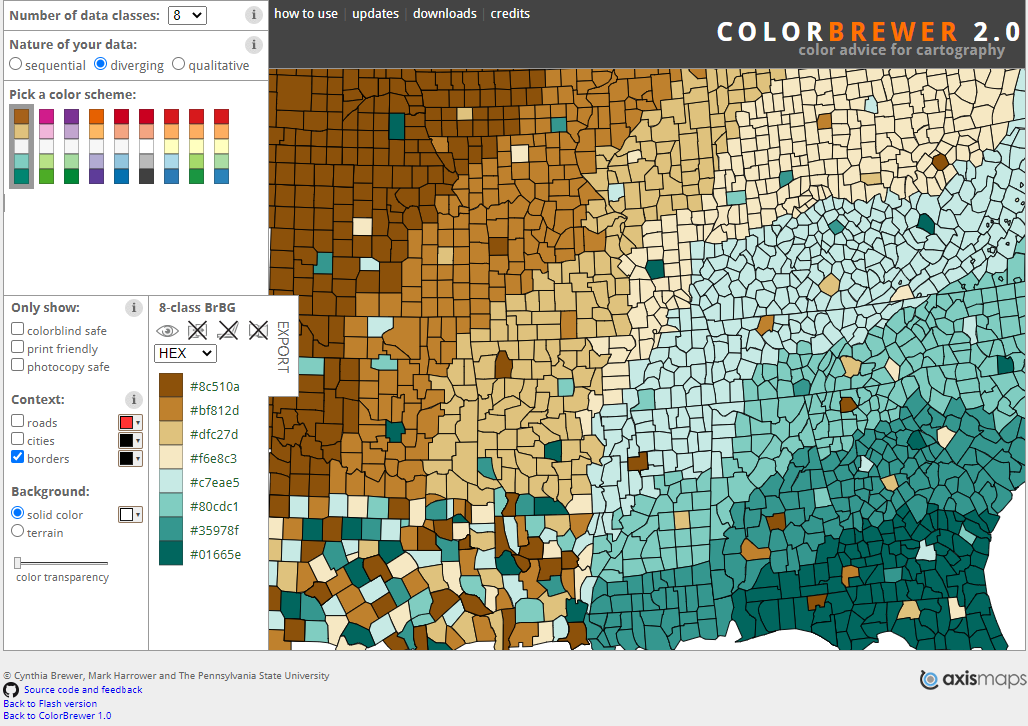
\includegraphics[width = 0.6\textwidth]{M5-ColourBrewer.PNG} \\  }
   \only<1>{\textcolor{gris}{\footnotesize{Source: \href{https://colorbrewer2.org/}{ColourBrewer}}} \\ }
   \only<2>{Choosing color with logic \\ }
   \only<2>{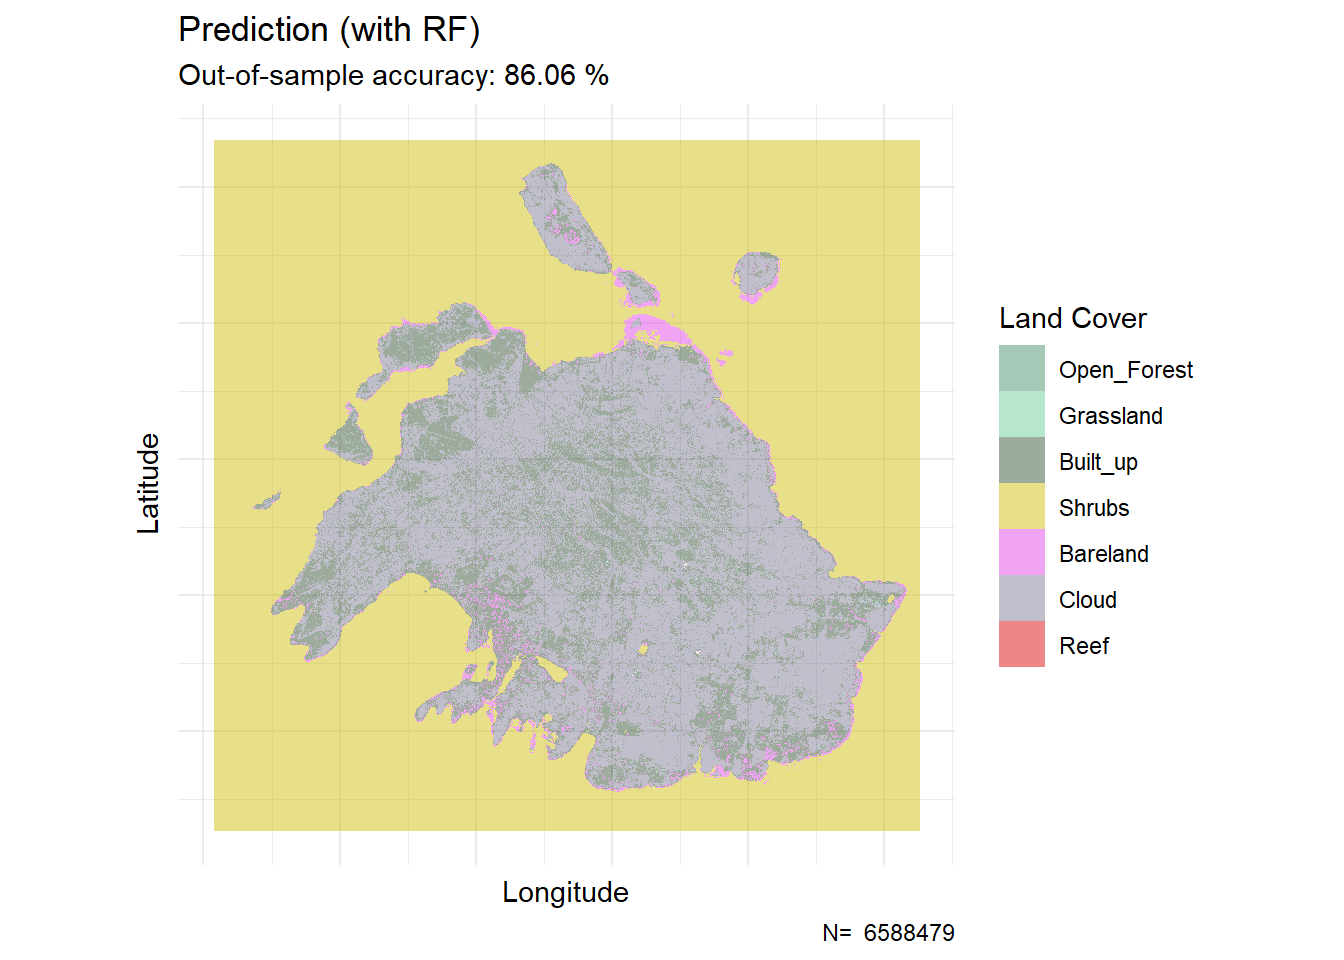
\includegraphics[width = 0.45\textwidth]{Paella-Vanuatu-Yellow.png} 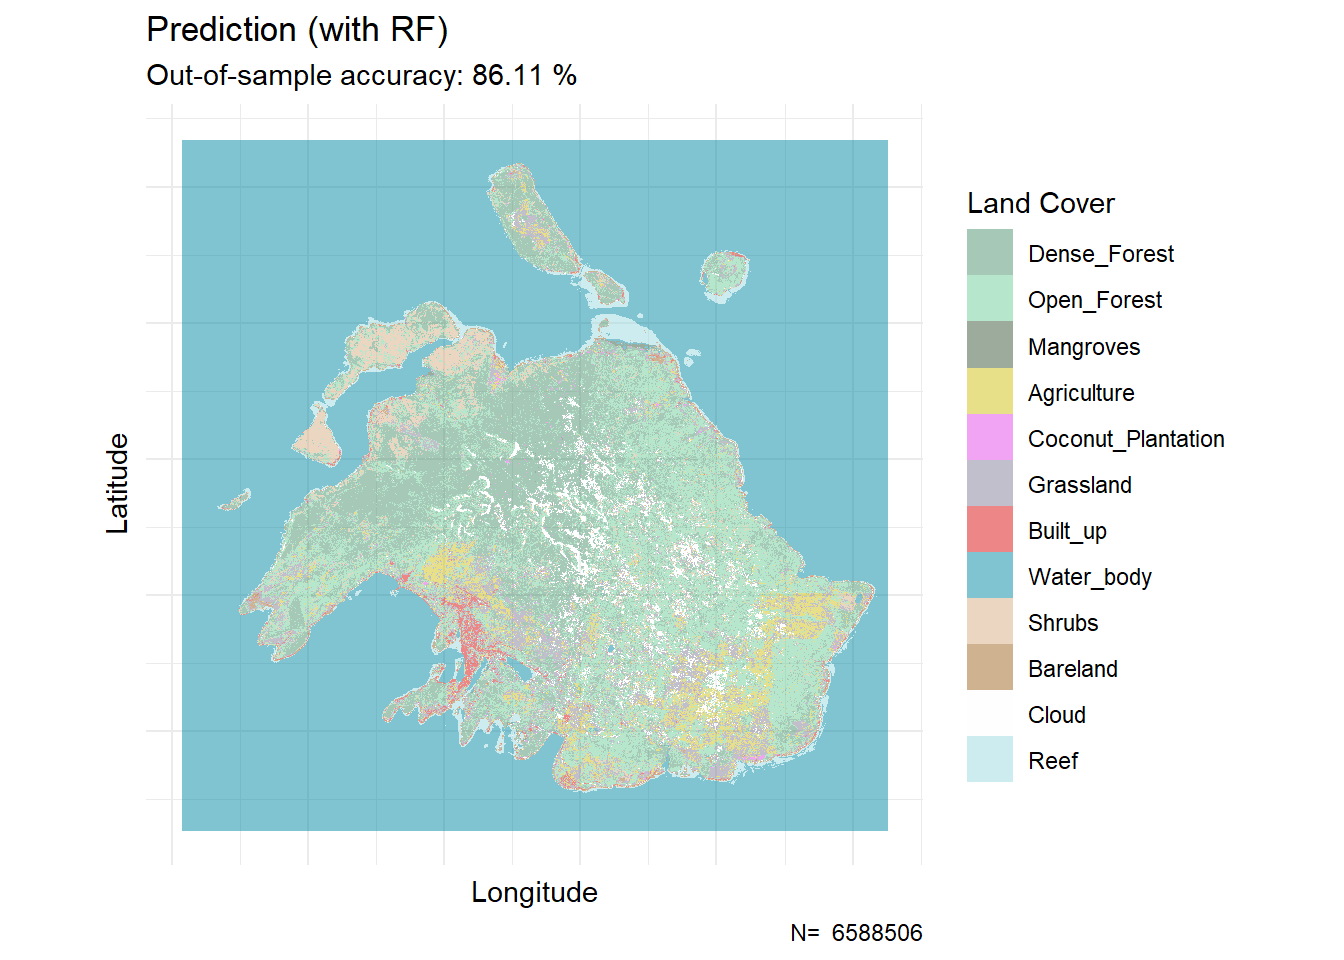
\includegraphics[width = 0.45\textwidth]{Paella-Vanuatu-RF.png}\\   }
   \only<3>{Colour is also cultural}
   \only<3>{\includegraphics[width = 0.8\textwidth]{ColorWheelCultural.png} \\   }
   \only<3>{\textcolor{gris}{\footnotesize{Source: \href{https://www.informationisbeautiful.net/visualizations/colours-in-cultures/}{Information is beautiful}}} \\ }
   \only<4-5>{Keep the focus on what is important}
   \only<4>{\includegraphics[width = 0.7\textwidth]{UNWomen-WomenPolitics2025.png} \\   }
   \only<5>{\includegraphics[width = 0.5\textwidth]{UNWomen-WomenPolitics2025-AP.png} \\   }
   \only<4-5>{\textcolor{gris}{\footnotesize{Source: \href{https://www.ipu.org/resources/publications/infographics/2025-03/women-in-politics-2025}{IPU-UN Women}}} \\ }
\end{itemize}
\end{center}
\end{frame}


\subsection{Limitations}

%\begin{frame} % Cover slide
%\frametitle{\textcolor{brique}{[-  \textbf{Choropleth maps  limitations} -]}}
%\begin{frame} % Cover slide
%\frametitle{\textcolor{brique}{[-  \textbf{Germany election map example} -]}}
%\begin{center}
%\begin{itemize}
%   \only<1>{Main result: \\ }
%   \only<1>{\includegraphics[width = 0.5\textwidth]{GermanElections.JPG} \\  }
%   \only<2>{Looking more closely:\\ }
%   \only<2>{\includegraphics[width = 0.9\textwidth]{GermanElectionsStackedBar.JPG} \\  }
%   \only<3-6>{Party by party: \\ }
%   \only<3>{\includegraphics[width = 0.5\textwidth]{GermanElectionsCDU.JPG} \\  }
%   \only<4>{\includegraphics[width = 0.5\textwidth]{GermanElectionsSPD.JPG} \\  }
%   \only<5>{\includegraphics[width = 0.5\textwidth]{GermanElectionsLINKE.JPG} \\  }
%   \only<6>{\includegraphics[width = 0.5\textwidth]{GermanElectionsAFD.JPG} \\  }
%   \only<7>{Small multiple solution \\}
%   \only<7>{ \centering
%            \includegraphics[width = 0.3\textwidth]{GermanElections.JPG} \\
%            \includegraphics[width = 0.2\textheight]{GermanElectionsCDU.JPG}
%            \includegraphics[width = 0.2\textheight]{GermanElectionsSPD.JPG}
%            \includegraphics[width = 0.2\textheight]{GermanElectionsLINKE.JPG}
%            \includegraphics[width = 0.2\textheight]{GermanElectionsAFD.JPG} \\ }
%   \only<1-7>{\textcolor{gris}{\footnotesize{Source: \href{https://flourish.studio/examples/german-elections/}{Flourish Studio}}} \\ }
%\end{itemize}
%\end{center}
%\end{frame}


\begin{frame} % Cover slide
\frametitle{\textcolor{brique}{[-  \textbf{Choropleth maps limitations} -]}}
\begin{itemize}[<+-|alert@+>]
    \item Choropleth maps are based on surfaces
    \item The \textbf{shape} of the visual variable is not homogenous
    \item The \textbf{surface} of the visual variable has no relation with the indicator that is encoded
\end{itemize}
\end{frame}

\begin{frame} % Cover slide
\frametitle{\textcolor{brique}{[-  \textbf{Land doesn't vote} -]}}
\begin{center}
\begin{itemize}
   \only<1>{Main result of a \textbf{\textcolor{airforceblue}{yes}-\textcolor{brique}{no} }question in Switzerland: \\ }
   \only<1>{\includegraphics[width = 0.7\textwidth]{M5-SwissChoropleth.JPG} \\  }
   \only<2>{The majority of the land is blue:\\ }
   \only<2>{\includegraphics[width = 0.8\textwidth]{M5-SwissChoroplethLand.JPG} \\  }
   \only<3>{But land don't vote (people do!) \\ }
   \only<3>{\includegraphics[width = 0.8\textwidth]{M5-SwissBubles.png} \\  }
   \only<4>{But land don't vote (people do!) $\hookrightarrow$ \textbf{\textcolor{brique}{no}} wins\\ }
   \only<4>{\includegraphics[width = 0.8\textwidth]{M5-SwissChoroplethVotes.JPG} \\  }
   \only<1-4>{\textcolor{gris}{\footnotesize{Source: \href{https://github.com/zumbov2/votemapswitzerland}{David Zumbach}}} \\ }
\end{itemize}
\end{center}
\end{frame}

\section{Proportional symbols}

\begin{frame} % Cover slide
\frametitle{\textcolor{brique}{[-  \textbf{Proportional symbols maps} -]}}
  \begin{columns}
  \column{0.6\textwidth}
    \begin{itemize}[<+-|alert@+>]
        \item Use a symbol, its shape and size to encode information
        \item The shape and it size is a \textbf{data-driven choice}
        \item We have some control, and choices are ours!
            \begin{itemize}[<+-|alert@+>]
                \item  Size
                \item  Position
                \item  Transparency
                \item  Color, scope, etc...  % Bahoken
            \end{itemize}
        \end{itemize}
     \column{0.4\textwidth}
        \includegraphics[width = 1.0\textwidth]{ShareWomenParliamentSymb-Small.png}
    \end{columns}
\end{frame}



\begin{frame} % Cover slide
\frametitle{\textcolor{brique}{[-  \textbf{Share of Women in Parliament} -]}}
\begin{itemize}
    \item[]
   \only<1>{Choice: \textbf{Type} of map: Choropleth vs symbols \\ }
   \only<1>{\includegraphics[width = 0.45\textwidth]{ShareWomenParliamentChoroCont.png}   }
   \only<1>{\includegraphics[width = 0.45\textwidth]{ShareWomenParliamentSymb-Small.png} \\  }

   \only<2>{Choice: \textbf{Size} of proportional symbol \\ }
   \only<2>{\includegraphics[width = 0.45\textwidth]{ShareWomenParliamentSymb-Big.png}   }
   \only<2>{\includegraphics[width = 0.45\textwidth]{ShareWomenParliamentSymb-Small.png} \\  }

   \only<3>{Choice: \textbf{Shape} of proportional symbol \\ }
   \only<3>{\includegraphics[width = 0.45\textwidth]{ShareWomenParliamentSymb-Square.png}   }
   \only<3>{\includegraphics[width = 0.45\textwidth]{ShareWomenParliamentSymb-Bar.png} \\  }

   \only<4>{Choice: \textbf{ Mixing} color (hue) and shape \\ }
   \only<4-5>{\includegraphics[width = 0.45\textwidth]{ShareWomenParliamentSymb-SquareColor.png}   }
   \only<4-5>{\includegraphics[width = 0.45\textwidth]{ShareWomenParliamentSymb-CircleColor.png} \\  }

   \only<5-6>{Is this the \textbf{best} way?  \\ }
   \only<6>{\includegraphics[width = 0.6\textwidth]{ShareWomenParliamentSymb-Gauge.png} \\  }
   \only<7>{ Or maybe, no maps?   \\ }
   \only<7>{\includegraphics[width = 0.55\textwidth]{ShareWomenParliament-BarChart.png} \\  }
   \only<6-7>{\textcolor{gris}{\footnotesize{Source: \href{https://freerangestats.info/blog/2023/05/26/women-parl-map}{Free Range Statistics}}} \\ }
  \only<8>{ Another Solution: Visualize \textbf{Men} in parliament \\ }
    \only<8>{ \includegraphics[width =0.5\textwidth]{MenInParliament.png} }
    \only<9>{ Another another solution: Use \textbf{both} a map and Bars \\}
    \only<9>{ \includegraphics[width =0.40\textwidth]{MenInParliament.png} \includegraphics[width =0.50\textwidth]{MenInParliamentBarChart.png} \\ }

\end{itemize}
\end{frame}


\subsection{Exercise}
\begin{frame} % Cover slide
\frametitle{\textcolor{brique}{[-  \textbf{Choices for a Maps} -]}}
\begin{center}
    \Large{\textcolor{siap}{The choices of symbols and colors affect \\
     \textbf{the reader's perception} of the message}} \\ \vspace{0.5cm}

    \large{\textcolor{siap}{\textit{$\hookrightarrow$
    \href{https://observablehq.com/@xtopheb/visualizing-statistics-on-maps}{Illustration with the Syrian migration in 2015}}}} \\ \vspace{0.5cm}
     \href{https://observablehq.com/@xtopheb/visualizing-statistics-on-maps}{\includegraphics[width = 0.4\textwidth]{Syrians-MapSize1.png}}\\
     \hfill\textcolor{gris}{ \footnotesize{Inspired by \href{https://neocarto.github.io/syrians/}{Françoise Bahoken \& Nicolas Lambert}}}
\end{center}
\end{frame}

%\begin{frame} % Cover slide
%\frametitle{\textcolor{brique}{[-  \textbf{Choice of symbols attributes} -]}}
%\begin{center}
%\begin{itemize}
%   \only<1> {\centering
%    \Large{\textcolor{siap}{The choices of symbols and colors affect \\
%     \textbf{the reader's perception} of the message}} \\
%     \vspace{1cm}
%    }
%   \only<1>{\centering
%    \large{\textcolor{siap}{\textit{Illustration with the Syrian migration in 2015}}} \\
%    }
%   \only<2>{\textbf{Size} of the circles: Small   \\
%   $ \;$  \\ }
%   \only<2>{\includegraphics[width = 0.9\textwidth]{Syrians-MapSize1.png}\\  }
%   \only<3>{\textbf{Size} of the circles: Medium    \\
%   $ \;$  \\ }
%   \only<3>{\includegraphics[width = 0.9\textwidth]{Syrians-MapSize2.png}\\  }
%   \only<4>{\textbf{Size} of the circles: Large    \\
%   $ \;$  \\ }
%   \only<4>{\includegraphics[width = 0.9\textwidth]{Syrians-MapSize3.png}\\  }
%   \only<5>{\textcolor{brique}{Colour} of the circles: Peaceful    \\
%   $ \;$  \\ }
%   \only<5>{\includegraphics[width = 0.9\textwidth]{Syrians-MapColor1.png}\\  }
%   \only<6>{\textcolor{brique}{Colour} of the circles: Aggressive    \\
%   $ \;$  \\ }
%   \only<6>{\includegraphics[width = 0.9\textwidth]{Syrians-MapColor2.png}\\  }
%   \only<7>{\textcolor{brique}{Colour} of the circles: Neutral     \\
%   $ \;$  \\ }
%   \only<7>{\includegraphics[width = 0.9\textwidth]{Syrians-MapColor3.png}\\  }
%   \only<8>{\textbf{Words} are important too...    \\
%   $ \;$  \\ }
%   \only<8>{\includegraphics[width = 0.9\textwidth]{Syrians-MapColor3-Invasion.png}\\  }
%   \only<9>{Combining size, colour and words: Welcome version    \\
%   $ \;$  \\ }
%   \only<9>{\includegraphics[width = 0.9\textwidth]{Syrians-MapCombine1.png}\\  }
%   \only<10>{Combining size, colour and words: Warning version   \\
%   $ \;$  \\ }
%   \only<10>{\includegraphics[width = 0.9\textwidth]{Syrians-MapCombine2.png}\\  }
%   \only<11>{The choice of the scope is important too!  \\
%   $ \;$  \\ }
%   \only<11>{\includegraphics[width = 0.8\textwidth]{SyriansMapDeZoomed.JPG} \\  }
%   \only<12>{The big picture  \\
%   $ \;$  \\ }
%   \only<12>{\includegraphics[width = 0.9\textwidth]{Syrians-BigMap.png} \\  } \only<2-12>{\textcolor{gris}{\footnotesize{Source: \href{https://neocarto.github.io/syrians/}{Françoise BAHOKEN \& Nicolas LAMBERT} }} \\ }
%\end{itemize}
%\end{center}
%\end{frame}


\section{New geometries}

\begin{frame} % Cover slide
\frametitle{\textcolor{brique}{[-  \textbf{New geometries: Cartograms}-]}}
\begin{center}
\begin{itemize}
   \only<1>{ }
   \only<2>{ \centering
    \large{\textcolor{siap}{A cartogram is a map with surfaces distorted by a continuous variable (DGP, Population).}} \\
   }
   \only<3>{\includegraphics[width = 0.5\textwidth]{M5-Cartogram_Africa1.PNG} \\  }
   \only<4>{\includegraphics[width = 0.5\textwidth]{M5-Cartogram_Africa2.PNG} \\  }
   \only<3-4>{ \hfill \textcolor{gris}{\footnotesize{Source: \href{https://www.r-graph-gallery.com/cartogram.html}{Yan Holtz-  From-Data-to-Viz}}} \\ }
   \only<5>{Other types of cartograms (weighting by GDP) \\ }
   \only<5>{\includegraphics[width = 0.5\textwidth]{M5-IndiaGDP-Geo.PNG} \\  }
   \only<6>{Continuous cartogram\\ }
   \only<6>{\includegraphics[width = 0.5\textwidth]{M5-IndiaGDP-Carto.PNG} \\  }
   \only<7>{Dorling\\ }
   \only<7>{\includegraphics[width = 0.5\textwidth]{M5-IndiaGDP-Dorling.PNG} \\  }
   \only<8>{Hexagonal Tiling \\ }
   \only<8>{\includegraphics[width = 0.5\textwidth]{M5-IndiaGDP-Hex.PNG} \hfill \textcolor{gris}{\footnotesize{Source: \href{https://atlan.com/courses/introduction-to-gis-r/lesson4-animated-interactive-maps/\#gis-ch4-nom_gdp_anim}{Sean Angiolillo}}} \\ }
\end{itemize}
\end{center}
\end{frame}

\begin{frame} % Cover slide
\frametitle{\textcolor{brique}{[-  \textbf{New geometries}-]}}
\begin{itemize}
   \item  \textit{Voxels} or \textit{Spike} maps   %https://static.geotribu.fr/articles/2020/2020-09-20_tutorial_aerialod/
    \item  Cartograms  % https://worldmapper.org/covid-19-coronavirus/  %https://blog.datawrapper.de/cartograms/
    \item  Tiles, Hex, Dorling,  and squares maps
    %https://atlan.com/courses/introduction-to-gis-r/lesson4-animated-interactive-maps/
\end{itemize}
\end{frame}



%\begin{frame} % Cover slide
%\frametitle{\textcolor{brique}{[-  \textbf{New geometries} -]}}
%\begin{center}
%\begin{itemize}
%   \only<1-3>{Population per square mile per state \\ }
%   \only<1>{\includegraphics[width = 0.9\textwidth]{UsaMap1.png} \\  }
%   \only<2>{\includegraphics[width = 0.9\textwidth]{UsaMap-Cartogram.jpeg} \\  }
%   \only<3>{\includegraphics[width = 0.9\textwidth]{USAMap-proportionalSymbolCartogram.png} \\ }
%   \only<4>{\includegraphics[width = 0.8\textwidth]{USAMap-Choropleth.jpg} \\   }
%   \only<1-4>{\textcolor{gris}{\footnotesize{Source: \href{http://blog.visual.ly/you-are-here-using-maps-in-data-visualization/}{Rockcontent}}} \\ }
%   \only<5>{\includegraphics[width = 0.9\textwidth]{USAMap-SpikePop.png} \\   }
%   \only<5>{\textcolor{gris}{\footnotesize{Source: \href{https://blog.datawrapper.de/spikemaps/}{Lisa Charlotte Rost}}} \\ }
%   \only<6>{Poverty rate in a \textit{squared} world \\ }
%   \only<6>{\includegraphics[width = 0.9\textwidth]{M3-PovertyMapSquares2017.JPG} \\  }
%   \only<6>{\textcolor{gris}{\footnotesize{Source: \href{https://datatopics.worldbank.org/sdgatlas/goal-1-no-poverty/}{SDG Atlas (world bank)}}} \\ }
%\end{itemize}
%\end{center}
%\end{frame}


%
%\begin{frame} % Cover slide
%\frametitle{Another solution : proportional symbol cartogram}
%\begin{figure}[h]
%\includegraphics[width = 0.8\textwidth]{UsaMap-SmallStates.jpeg}
%\caption{Population per square mile per state (2000 census)}
%\end{figure}
%\footnotesize{\texttt{http://blog.visual.ly/you-are-here-using-maps-in-data-visualization/}}
%\end{frame}
%

 \section{Conclusion}

\begin{frame}
\frametitle{\textcolor{brique}{[-  \textbf{In conclusion }-]}}
\begin{itemize}[<+-|alert@+>]
    \item Communicating Gender Statistic with Maps is difficult!
    \item Statistical maps are useful and reveal spatial patterns
    \item Statistical maps follow rules
    \item There are good tools and tutorials
\end{itemize}
\end{frame}

\begin{frame}
\frametitle{\textcolor{brique}{[-  \textbf{In conclusion }-]}}
\begin{itemize}[<+-|alert@+>]
    \item Good example exist! $\hookrightarrow$  \href{https://datatopics.worldbank.org/sdgatlas/goal-1-no-poverty?lang=en}{\textbf{Atlas of SDGs 2020- 2023}}
    \item[]
    \includegraphics[width = 0.45\textwidth]{PovertyMapSquares1996.PNG}
    \includegraphics[width = 0.45\textwidth]{PovertyMapSquares2017.PNG} \\
     \hfill \includegraphics[width = 0.20\textwidth]{PovertyMapSquaresLegend.PNG} \\
   \textcolor{gris}{\footnotesize{Source: \href{https://datatopics.worldbank.org/sdgatlas/archive/2020/goal-1-no-poverty/}{World bank Atlas of SDGs 2020}}}
  \item Not all geospatial data should be maps

\end{itemize}
\end{frame}


%%%---- References---- %%%%
%%  \section{References}

% the \setbeamercolor and the frame to limit the scope
{\setbeamercolor{background canvas}{bg=siap}
 \setbeamercolor{item}{fg=white}
    \setbeamercolor{normal text}{fg=white}
    \usebeamercolor[fg]{normal text}

\begin{frame} % Cover slide
\hspace{4cm}
\begin{center}
\Huge{References}
\nocite{brewer1994}
\nocite{krygier2016}
\nocite{Monmonier2018}
\nocite{nusrat2016}
%\nocite{wilkinson1999}

\end{center}
%\footnotesize{source: \texttt{ https://upload.wikimedia.org/wikipedia/commons/0/0a/Semaphore_Signals_A-Z.jpg/}}
\end{frame}


\begin{frame}[allowframebreaks]%in case more than 1 slide needed
\frametitle{References}
    {\footnotesize
    %\bibliographystyle{authordate1}
    \bibliographystyle{apalike}
    \bibliography{Visu, VisuSeminal}
    }
\end{frame}

\end{document} 